\documentclass[12pt]{article}
	\usepackage[T1]{fontenc}
	\usepackage[utf8]{inputenc}
	\usepackage[british]{babel}
	\usepackage[a4paper]{geometry}
	\geometry{verbose,tmargin=3cm,bmargin=3cm,lmargin=2cm,rmargin=2cm,marginparwidth=70pt}
	\setcounter{secnumdepth}{3}
	\setcounter{tocdepth}{3}
	\setlength{\parindent}{4em}
	\setlength{\parskip}{1em}
	\renewcommand{\baselinestretch}{1.5}
	\usepackage{prettyref}
	\usepackage{textcomp}
	\usepackage{booktabs}
	\usepackage{lscape}
	\usepackage{setspace}
	\usepackage{indentfirst}
	\usepackage{fancyhdr}
	\usepackage{url}
	\usepackage[normalem]{ulem}
	\usepackage[table, fixpdftex]{xcolor}
	\usepackage{algpseudocode}
	\usepackage{bigstrut}
	\usepackage{enumitem}
	\usepackage{verbatim}
	\usepackage{mathtools}
	\usepackage{graphicx}
	\usepackage{longtable}
	\usepackage{chngpage}
	\usepackage{pdfpages}
	\usepackage{rotating}
	\usepackage{adjustbox}
	\usepackage[toc,page,title]{appendix}
	\usepackage[super]{nth}
	\usepackage[all]{nowidow}
	\usepackage{ragged2e}
	\usepackage[font=scriptsize,labelfont=bf]{caption}
	\DeclareCaptionLabelFormat{blank}{}
	% package hyperref
    \usepackage[hidelinks]{hyperref}
  

	% biblatex
	\usepackage[style=authoryear,natbib=true,maxcitenames=2,maxbibnames=11,backend=biber,pagetracker=page,hyperref=true]{biblatex} 
	\usepackage{csquotes}
	\renewcommand*{\bibsetup}{%
		\interlinepenalty=10000\relax % default is 5000
		\widowpenalty=10000\relax
		\clubpenalty=10000\relax
		\raggedbottom
		\frenchspacing
        \biburlsetup}
        
	% fixes the page number of the first page of each chapter
	\fancypagestyle{plain}{
			\fancyhead{}
			\renewcommand{\headrulewidth}{0pt}
			\renewcommand{\footrulewidth}{0pt}
			\fancyfoot[OC]{\begin{flushright}\thepage\end{flushright}}
    }
    
	% fancy headers for the thesis
	\fancyhead{}
	\fancyhead[RO]{\slshape \nouppercase \rightmark}
	\fancyfoot[OC]{\begin{flushright}\thepage\end{flushright}}
	\renewcommand{\headrulewidth}{0.4pt}
	\setlength{\headheight}{14pt}

	% add bibliography database
	\addbibresource{BA copy.bib}
	
	% space between biblio items
	\setlength\bibitemsep{1.7\itemsep} 
	
	% title without ""
	\DeclareFieldFormat[inbook]{title}{#1}
	% non-italic
	\DeclareFieldFormat[online]{tlaitle}{#1} 
	% title unquoted
	\DeclareFieldFormat[article]{title}{#1} 
	% no pp. 
	\DeclareFieldFormat[article]{pages}{#1} 
	% bold volume
	\DeclareFieldFormat*{volume}{\mkbibbold{#1}\setpunctfont{\textbf}}
	
	% no in:
	\renewbibmacro{in:}{} 
	
	% (volume)
	\renewbibmacro*{volume+number+eid}{%
			\printfield{volume}%
			%\setunit*{\adddot}% DELETED
			% \setunit*{\addnbspace}% NEW (optional); there's also \addnbthinspace
			\printfield{number}%
			% \setunit{\addcomma\space}%
			\printfield{eid}}
	\DeclareFieldFormat[article]{number}{\mkbibparens{#1}} 
	
	% edition.
	\DeclareFieldFormat{edition}%
	{(\ifinteger{#1}%
			{\mkbibordedition{#1}\addthinspace{}ed.}%
			{#1\isdot}).}
	
	% publisher and location p osition
	\renewbibmacro*{publisher+location+date}{%
			\printlist{publisher}%
			\setunit*{\addcomma\space}%
			\printlist{location}%
			\setunit*{\addcomma\space}%
			\usebibmacro{date}%
			\newunit}
	
	% shortauthor before author
	\renewbibmacro*{begentry}{%
			\ifkeyword{Key}{\sffamily}{}%
			\iffieldundef{shorthand}
			{}
			{\global\undef\bbx@lasthash
					\printfield{shorthand}%
					\addcolon\space}%
			\ifboolexpr{test {\usebibmacro{bbx:dashcheck}} or test {\ifnameundef{shortauthor}}}%
			{}%
			{\printnames{shortauthor}%
                    \addspace\textendash\space}}
                    
\title{Does Financial Constraints of Corporate Activist Investors Matter?}
\author{Leopold Ingenohl}


\begin{document}
\begin{titlepage}
    \begin{center}
       
        
\includegraphics[width=0.5\textwidth]{Logo.jpg}
       
        \vspace*{1.5cm}
		\huge
        \textbf{Do Financial Constraints of Corporate Activist Investors Matter?}

        \vspace{1.5cm}
		\normalsize
        Leopold Ingenohl\\
        Richard-Wagner Str. 7\\
        76185, Karlsruhe\\
        leopold.ingenohl@student.unisg.ch\\
        15-613-631

        \vspace{1.5cm}
        Supervised by:\\
        Prof. Dr. Markus Schmid\\
        Swiss Institute of Banking and Finance (s/bf)\\
        \vfill

        A thesis presented for the degree of\\
        Bachelor of Arts HSG

        \vspace{0.8cm}

        Submitted May xx, 2018

	\end{center}
	
\end{titlepage}

\tableofcontents
\listoftables
\listoffigures
\pagebreak

\section{Introduction}

If any person acquires beneficial ownership of more than 5\% of an issuer's securities he must file with the Stock Exchange Control (SEC) a Schedule 13(D) within 10 days after the acquisition of that stock. The crux herein lies in beneficial ownership which is not defined as whether the person owns the shares but as whether the particular person can vote the shares and thereby change or influence the control of the company \citep[p.24]{Morrison2015}. Precisely this mindset is what constitutes shareholder activism, independent of the acquirers identity. In fact, a Schedule 13(D) has to be disclosed by most investor types such as individuals, hedge funds and corporations. In the words of \citet[p.187]{Klein2009}, an "entrepreneurial activist is an investor who buys a large stake in a publicly held corporation with the intention to bring about change and thereby realize a profit on the investment". Complementary thereto, corporations filing a Schedule 13(D) to deliberately practice their voting power can be classified as corporate activist investors. 

Hedge fund activists seek to gain seats on the company's board, oppose an existing merger or liquidation of the firm, pursue strategic alternatives or replace the CEO \citep[p.188]{Klein2009}. Motivation for corporate activist investors to acquire beneficial ownership is to overcome informational and integration barriers and thereby engage in proceedings such as takeovers and strategic cooperations \citep[p.1]{Huang2017}. Strategic minority acquisitions help reduce holdup costs, mitigate financing constraints and facilitate greater innovation and relation-specific investment \citep[p.825]{Wang2014}. In turn, they are followed by significant benefits for both firms \citep[p.2793]{Allen2000}.

This action for change is mirrored by a positive market reaction at the announcement of the filing. Hence, when an investor's Schedule 13(D) filing becomes public, the firm that has been partially acquired experiences significant gains on its stock. In recent studies of what happens to the target's stock, \citet[p.1564]{Collin-Dufresne2015} find significant positive abnormal returns around the filing day for filings of all investor types. The evidence is consistent with \citet[p.1756]{Brav2008} and \citet[p.209]{Klein2009} who report 8.4\% and 7.2\% abnormal returns respectively but in response to hedge fund activism. The only study inexplicitly noting a positive market reaction to corporate activist investors is by \citet[p.29]{Brigida2012}. This study finds evidence on this matter, as targets of corporate activist investors from the sample experience 14\% average abnormal returns around the filing date of the Schedule 13(D). The positive market reaction is consistent with the evidence of the market's anticipation that activism, likewise action for change, results in actual value improvement for the target \citep[p.1760]{Brav2008}.\\
The possible increase in value however, is dependent on the initiator of activism, as it is their own effort that brings the change \citep[p.1563]{Collin-Dufresne2015}. So if the initiator of activism stands for the actual value improvement, its ability to finance action for change and further involvement in the target, especially in the case of corporate activists, should be related to the market's evaluation of the target's potential gains.

A recent example on this matter is the public's perception of China's largest private conglomerate, the HNA Group. Over the past few years they invested around \$US40 billion in businesses around the world and have currently been of great interest to financial news \citep{Smith2018}. Not least because they built up a 9.9\% stake of of around \$US4 billion in Deutsche Bank in 2017, but also because of their complex and nontransparent financing methods \citep{Lockett2018}.
The financing of the group has come under strain as a result of an official crackdown on risky financing at acquisitive private enterprises in China. The highly leveraged group is now facing a potential cash-shortfall and liquidity issues resulting in a S\&P global rating downgrade referring to a a „deteriorating liquidity profile" of HNA \citep{Schuetze2018}. Although the HNA Group is a private conglomerate, the financial appearance of the investor seems to be of great interest to other market participants. The Schedule 13(D) on 28 April, 2018 in which they announced their 9.9\% stake in Deutsche Bank was followed by an increase in Deutsche Bank's value. This said, had the increase in value of Deutsche Bank been larger with an HNA Group financially less constrained and thereby more assertive? Hence do financial constraints of corporate activist investors matter when the market anticipates a possible value improvement for the target?\\ 
As financially unconstrained corporations are able to raise substantial amounts of external capital, thereby signalising the capability of further involvement in any form and embodying the potential for change, the opposite should be true for financially constrained firms \citep[p.1]{Farre-mensa2013}. Following, the anticipated value improvement should be less for financially constrained firms if the assumption holds that the actual value improvement for the target is dependent on the ability of the investor to bring change.
This thesis finds evidence that it does. The univariate tests show that targets of financially constrained corporations gain less when compared to targets of unconstrained investors. For instance, when financially constrained investors are identified by using the Whited-Wu index, the target's abnormal return is on average 10\% higher had they been unconstrained. They have average abnormal returns of around 6\% whereas targets of financially unconstrained firms experience average abnormal returns of around 16\%. The significant difference of 10\% in abnormal returns indicates that financial constraints of corporate activists investors matter. The multivariate analysis confirms that, other things being equal, the financial constraints of the investor are an important determinant of the abnormal returns of the target. Targets of constrained investors earn 10\% less in the [-10,3] event-window indicating financial constraints of corporate activist investors matter, when the market perceives the actual value improvement for the target. 

The paper proceeds as follows. Section 2 reviews relevant literature on Schedule 13(D) filings, their effect on the market, corporate equity ownership and financial constraints. Section 3 outlines the composition of the sample and identifies the sample's corporate activist investors. Section 4 investigates the market's reaction to Schedule 13(D) filings and analyses the univariate relation between target's abnormal returns and investor's financial constraints while Section 5 evaluates the cross-sectional effect of financial constraints on the target's gains.

% Characteristics | Motivation | Reasoning - Why do they make minority acquisitions? 

% Topics: Acquisitions | Friendly Takeovers | Hostile Takeovers | Joint-Venture | Activism | Comparison | Comparison HF - Why do they behave activist? 
% In a more direct approach however, these strategic investments can also help as a stepping stone towards full control \citep{Huang2017}. 
% This approach is supported by \citet{Goldman2005} who find that mergers and takeovers are often preceded by the acquisition of a minority stake in the target. Whereas hedge funds use their stakes to change characteristics of the target (e.g. the board of directors or the strategic orientation) \citep{Klein2009} corporate filers are mainly focused on synergies in the form of strategic alliances or takeovers between them and the target. \citet{Akhigbe2007} observe that partial acquisitions, if carried out by corporate investors, are more likely to result in a full acquisition when compared to all other activist investors. This means that within the mass of Schedule 13D filings, institutional investors are unlikely to pursue a complete takeover whereas corporations are potential full acquirers \citep{Brigida2012}. The possibility of a takeover could be one explanation for the strong impact corporate filings have on the market, because the abnormal returns could be a reflection of investors' expectations of the target firms stock being acquired at a premium to the current price \citep{Goldman2005} especially with strong corporate bidders being likely to overpay in the event of a full takeover \citep{Akhigbe2007}.
% These findings motivate the second hypotheses which assumes the highest abnormal returns occur in the event of a purpose of transaction statement involving a merger or a takeover of the subject.
%Objective: highlight the importance of the financial condition -- Background

% payment method in takeovers! 

% Topics: Abnormal Returns | Financial Condition | Activism | Hypothesis | Conclusion
 



\begin{comment}
	\section{Hypotheses}

\begin{enumerate}
	\item There are significant positive abnormal returns after the Schedule 13(D) filing of a corporation
	\item The purpose of the transaction has an effect on the market reaction 
	\item The financial condition of the investor can explain the market reaction
	\item The financial condition is most important, when the puspose of transaction invovles a future merger or takeover
	\item The financial condition looses its importance when the target is a poorly performing company and gains importance when the target is performing well 
	\item 
\end{enumerate}
\end{comment}


\section{Literature Review}

\subsection{Schedule 13(D) Filings \& Market Reaction}
%Topics: Historical Background | Information contained | Difference G and D

Section 13(d) of the Exchange Act of 1934 was passed in order to increase regulation of tender offers and accumulations of stock.
It acts as an early warning, signaling "every large, rapid aggregation or accumulation of securities, regardless of technique employed, which might represent a potential shift in corporate control" \citep[p.2]{Morrison2015}. 
This means that under Section 13(d), anyone who becomes the beneficial owner of 5\% of an issuer's equity securities registered under Section 12 of the Exchange Act must file with the SEC a Schedule 13(D) within 10 days after the acquisition. The filing informs shareholder about investors who could influence or change control of the issuing company \citep[p.110]{Giglia2016}. The investors filing such a Schedule 13(D) can be broadly classified into institutional investors (e.g. hedge funds or mututal funds), other entrepreneurial activists (e.g. individual investors) \citep[p.188]{Klein2009} and relevant for this thesis, corporate investors. Amongst others, the filing specifies the security and the issuer subject to the filing, the identity and background of the filer, and the purpose of the transaction.\\
Whereas filing a Schedule 13(D) allows the investor to practice its voting power in an active manner, a passive investor can equivalently file a Schedule 13(G). It is a short-form filing that can be utilized if an investor holds a beneficial ownership interest passively, with no intent to change control of the company \citep{Giglia2016}. Therefore, corporations filing a Schedule 13(D) confess to manage their investments actively, likewise confess to approach and interact with the target company and can therefore be called corporate activist investors. 
%Topics: Characteristics AR | Problems in Comparison | Motivation of HF | Activism

So far, there exist many studies that examine the effect the disclosure of such an activist investment has on the target's stock. With regards to short-horizon event studies, all these studies find positive and significant abnormal returns around the Schedule 13(D) filing date.\\ 
Dealing with investor activism, especially filings disclosed by hedge funds, \citet[p.1730]{Brav2008} find positive average abnormal returns in the range of 7\% to 8\% in the (-20,+20) event window. \citet[p.188]{Klein2009} have similar findings and observe 10.2\% average abnormal stock returns on the target's stock. In a more recent study on investor activism by \citet[p.410]{Denes2017}, the average valuation effect is evaluated to be around 5\%. A somehow different approach is found in a study of \citet[p.363]{Greenwood2009} who observe abnormal announcement returns of 2.36\% for a sample of activist portfolio investors and document that the ability to force the target into a takeover is the driving force behind the abnormal market reaction. Nevertheless, all studies observe positive abnormal returns around the filing date and results only differ in magnitude.\footnote{Comparing the the abnormal returns across studies can be misleading as the authors used different models and event windows for estimating the abnormal returns. \citet{Greenwood2009} use the market return model with matching portfolios and the CAR for aggregated abnormal returns; \citet{Brav2008} calculates the aggregated abnormal returns by subtracting the value-weighted market index from the buy-and-hold return; \citet{Klein2009} use a similar approach with buy-and-hold returns but make more adjustments.}

While all of these studies identify hedge fund activism, its motivation and the effect it has on the market, most of them leave filings submitted by corporations aside. \citet[p.29]{Brigida2012} however, note that if the acquirer is a non financial corporation abnormal returns in the (-10,-1) window are around 14\%. The reaction implies the market perceives such corporate investments as value generating for target. \citet[p.2803]{Allen2000} find abnormal returns of around 7\% in the (-10,10) period on corporate purchase announcements which are significantly larger if the announcement is accompanied by strategic investments. Their sample however is based on purchase announcements and therefore differs from studies on the effect of Schedule 13(D) filings.\footnote{In \citet[p.2801]{Allen2000} sample, the mean fraction of equity acquired in the sample is 14\%, and includes acquisitions of at least 5\% of voting shares only.} In addition \citet{Collin-Dufresne2015} find a positive significant market reaction upon a more general sample of Schedule 13(D) filings, including corporate investors but not explicitly addressing them.\\
So what is the motivation of corporations to engage in active equity ownership, thereby disclosing a Schedule 13(D), and why are these investments anticipated to be value generating for the target?

% What is constrained, distressed? 
% Because financial distress possibly resulting in bankruptcy represents a state in which the firm cannot meet or has difficulty paying off its financial obligations to its creditors the reference to HNA Group made above is exemplary here as the group has problems in refinancing the enormously high debt burden. 



% Although the filing of a Schedule 13(D) can be seen as the trigger for the market reaction, the reason of why the abnormal returns occur is still largely unknown. However, \citet{Brav2008} find that if hedge funds engage actively, they have a high succession rate in achieving their main objectives. In a more recent paper conducted by \citet[p.12]{Brav2009} they list these objectives based on the sample of filings. The vast majority of these objectives focuses on general characteristics of the target and possible increase in shareholder value. They can be separated into five, not mutually exclusive, categories. The first objective is the believe of the hedge fund that he can help the manager maximize the shareholder value because they believe that the company is undervalued. The second includes activism that is based on the targeting firm's payout policy and capital structure. for the third objective, the hedge funds target issues related to business strategy, such as operational efficiency, mergers and acquisitions or growth strategies. The fourth objective is aimed at the sale of the target company with the majority to force a sale of the target company to a third party. The last objective includes activism targeting corporate governance. These motives are congruent with the \citet{Klein2009} definition of an entrepreneurial activist "who buys a large stake in a publicly held corporation with the intention to bring about change and thereby realize a profit on the investment". A more cautious definition is presented by \citet{Greenwood2009} who define an activist investor as someone who tries to change the status quo through voice, without a change in control of the firm. 

\subsection{Motives of Corporate Equity Ownership, Value Creation \& Financial Constraints}
% 13(D) = Minority Acquisition - Proxy 
%Topics: General Objectives | Definitions | Motivation | Minority Acquisitions | Toehold  

Corporate investments in other firms' equities can be be split into three broad categories. They can either be classified as ordinary, far more importantly as strategic and thirdly as stepping stones in a takeover process. 
In the sense of possibilities that might be reached, corporate ownership, in comparison to ownership by institutional investors, is unique \citep[p.2791]{Allen2000}.

\citet[p.1]{Huang2017} suggest that corporations make strategic minority acquisitions in other companies when they confront informational or integration barriers. 
Therefore, one reason for corporations to acquire a partial stake is that in the presence of alliances or joint ventures, minority acquisitions help to align the incentives of both firms involved and thereby decrease contracting and monitoring costs \citep[p.2792]{Allen2000}. This especially is of importance, if the strategic cooperation involves relationship specific assets and the investing corporation might be concerned with a holdup problem.\footnote{\citet[p.1023]{Ouimet2013} Defines the holdup problem as a decrease in the investors bargaining power in a renegotiation of the contract because the value of the initial investment is dependent on future cooperation with the target.} \citet[p. 2793]{Allen2000} show that in the years following a strategic investment,  targets increase investment expenditures, exhibit substantive gains in operating cash flow and the partial stake leads to significant benefits for both firms.\\
The second motive behind corporate minority investments is that if asymmetric information has an adverse effect on cost and availability of external capital for the target, the investment can provide capital directly to the issuing firm or validate its investment opportunities \citep[p. 2792]{Allen2000}. This is supported by \citet[p.1038]{Ouimet2013} who finds that the investment helps to overcome asymmetric information and thereby helps to certify the target for other outside investors. This proposition is verified by \citet[p.78]{Liao2014} who finds that target firms issue new equity (debt) and raise their market capitalization thereby supporting the theory that equity stakes certify the investment opportunities of target firms. Target firms correspondingly increase their operating cash flows, sales and investment expenditures.\\ 
Thirdly, by acquiring partial stakes, corporations can effectively monitor or influence the target's management. When compared to institutional investors, a corporate investor has superior knowledge and operating expertise \citep[p.2792]{Allen2000} and can thereby further increase the target's operational performance.\\
But acquiring a minority position also helps to better assess real options, notably that of expanding. The acquisition of a minority stake helps to better assess the target for a potential majority acquisition \citep{Ouimet2013} and according to \citet[p.30]{Huang2017} gather more information before launching a bid for takeover. In this sense, by decreasing informational barriers the investments can help as a stepping stone towards full control \citep[p.3]{Huang2017}.\\
Because there exist two options two acquire full control of a publicly traded firm in the United States, either through a merger or through a tender offer \citep[p.2]{Offenberg2015}, \citet[p.1]{Betton2008} use the term takeover "for any acquisition of corporate control through the purchase of the voting stock of the target firm, regardless of whether the bid is in the form of a merger agreement or a tender offer".
Prior to the takeover bid, the corporations can also acquire a toehold where neither management nor target's shareholders know of the investor's takeover intention until the announcement of a Schedule 13(D) is due \citet[p.158]{Eckbo2009}. Ultimately, takeovers are interlinked with offer premiums and target shareholders are compensated with premiums of around 45\% relative to the target share price \citep[p.154]{Eckbo2009}.\\
Concluding, corporations filing a Schedule 13(D) and thereby confessing to actively manage the investment have several reasons to do so. However, overcoming informational and integration barriers seems to pervade in almost all cases and there exists potential for actual value improvement. Strategic investments generate value through synergies, the target's financing validates investments opportunities and engaging in a takeover leads to offer premiums. So information contained in corporate Schedule 13(D) filings is of value to the market's target evaluation. 

But beyond the motives of corporations to actively engage in another firm and the benefits such an investment brings to both, to what extent does the corporations financial condition matter when the market values such activist investments?  While motives and benefits are conceivable, their successful implementation is dependent on the corporate investor. 
Thus if the investing company proxies for the target's value improvement, its financing capabilities should have an impact on the market's anticipation of present and future value of the target. At large, do financial constraints of corporate activist investors matter when the market reacts to Schedule 13(D) filings?\\
Under the assumption of perfect capital markets, the financial structure of the investor should be irrelevant to investment and the market, because "external funds provide a perfect substitute for internal capital" \citep[p. 141]{Fazzari1988}. This however, is not the case for financially constrained firms because they face an inelastic supply of external capital \citep[p.1]{Farre-mensa2013}. Hence, financial constraints refer to the degree of access to external financing. Consequently, firms who are able to raise substantial amounts of external capital without much of an increase in the cost of capital are considered as unconstrained \citep[p.1]{Farre-mensa2013}. This results in \citet[p.531]{Whited2006} measure of financial constraints, in which financial constraints affect the intertemporal substitution of investment today for investment tomorrow via the shadow price of scarce external funds -- their investment policy is dependent on the cost of capital. Because constrained firms have less access to external financing, \citet[p. 142]{Fazzari1988} argue that a constrained company's investment behavior is dependent on fluctuations in the companies cash flow and can therefore be unstable. As difficulties of external financing could also imply that the company is subject to information asymmetry, the quality of the investor's investment opportunities has not been evaluated comprehensively by providers of external finance \citep[p.142]{Fazzari1988}. Furthermore, constrained firms appear to invest at a low rate, despite good investment opportunities \citep[p.533]{Whited2006}. This means that financial constraints arise from friction such as information asymmetries that make external funds more costly than internal funds and lead to a different investment behavior compared to healthy firms. 
Following \citet[p.691]{Almeida2011a} a majority of managers in the U.S. list financial flexibility as the most important goal of their firm's financial policies which is consistent with the idea of of ensuring funding for future investment undertakings. This said, financial constraints of corporate activist investors should matter when the market evaluates the value improvement for the target.


% \citet[p.450]{Bhagat2005} investigate whether the same can be assumed about the investment policy of distressed firms and find it does. They also show that firms in distress invest less and "behave differently from financially constrained firms" \citep[p.461]{Bhagat2005}. 
% In addition, the size of the investing corporation could also play an important role in the market's investment valuation of the investment in the target. Large firms may enjoy easier access to capital markets, receive higher credit ratings for their debt issues and pay lower interest rates on borrowed funds \citep{Saquido2003}

% Considering the takeover process mentioned above, the necessity to file a Schedule 13(D) and thereby confirm the beneficial ownership of at least 5\% of the outstanding stock, prior or while negotiating the takeover bid, is more difficult to comprehend. Nevertheless the success of a potential takeover seems to be especially dependent on the bidders condition to be faster and stronger than potential competitors, the initial bidder has to ensure assertiveness. In order to appear strong (the market perceives the acquirer as a winner) the acquiring company must have sufficient financial strength. In the first place to make the takeover process credible to outside investors and secondly to signal the ability to pay the takeover premium. In any case, the target's outstanding shares have to be acquired at a premium to the price prevailing at the filing date either trough cash, stock or a mix of both. Besides that, a strong acquirer could have more bargaining power in persuading the target's shareholders to approve the merger and successfully carry out the takeover. 
% To faciliatate thhareholders of the target might sign a voting agreement in favor of the acquirer in which they agree to vote the shares in a way expressed by the acquirer - corporations might have to sign a Schedule 13(D) although they did not buy the shares but have their voting power.
% Whereas a merger agreement is the result of negotiations between the investor and the target's management, in a tender offer the acquirer makes a direct bid to target shareholders to purchase the target shares.
% By negotiating with the target's management a merger agreement might appear as the safer option. However, it does not lock up the target from potential competition because the director fiduciary duties require the target board to evaluate competing offers until the agreement is approved by the shareholders \citep{Mitchell2011}.  To prohibit the acquirer of purchasing target shares in the market during negotiations, parties often sign a standstill agreement \citep{Mitchell2011}.  
% Another possibility is the purchase of ownership in the target prior to the start of the takeover bid - a toehold. Neither management nor target's shareholders know of the acquirers takeover intention. Following \citet[p.158]{Eckbo2009} acquiring a toehold, before initiating the takeover bid, is compelling. It reduces the number of shares that must be bought at the full takeover premium and it can be sold at a profit if a rival bidder winds the target but it can also create hostility with the target's management \citep{Goldman2005}. This is the reason why toeholds are much more common in hostile bids \citep{Mitchell2011}. On the other hand \citet[p. 216]{Povel2014} suggest that toeholds are not much different to the general minority acquisitions. Because the toeholder might negotiate the right to nominate one or more directors in the target's board, they open the door to a more intensive cooperation. According to \citep{Mitchell2011} bidders initiating a takeover bid in the U.S. over the period 1980-2005 offered all cash as payment in 26\% of the cases, all stock in 37\%, and a mix of both in 37\%.
\section{Data -- Constructing the Sample}

The data that is used to analyse the relation between the investor's financial condition and the market reaction to Schedule 13(D) filings,  is primarily composed of information contained in the filings from SEC's Edgar database and secondly of data on stock and fundamentals,  accessed through Wharton Research Data Services (WRDS). The sample of Schedule 13(D) filings is constructed as follows. First, using an automated search script, 48'626 filings from the 20 year period starting in January 1996 and ending in December 2016 were identified.  The script identifies all Schedule 13(D) filings that appear on EDGAR and extracts the following information: name of filer and subject, the CUSIP of the underlying security and the filing date. Next, to only have filings submitted by corporations hence to separate corporate investors from institutional investors (i.e. hedge-funds or pension-funds), 10-K reports were cross-referenced with the initial sample of filings.\footnote{10-K reports were used to identify corporations because "managers of publicly traded firms are required to produce public documents that provide a comprehensive review of the firm’s business operations and financial condition and an important financial disclosure document created by managers to communicate with investors and analysts is the annual report filed pursuant to the Securities Exchange Act of 1934 the Form 10-K." \citep[p. 1643]{Loughran2014}} To be considered, the filer had to have a 10-K report submitted at least 12 months prior to the filing which reduced the sample to 3'325 filings. As daily stock returns and prices for the target's securities come from the Center for Research in Security Prices (CRSP) the subject not only had to have SEC's Cusip identifier but also an active link between Cusip and CRSP's Permno identifier. For estimating the market reaction to Schedule 13(D) filings, there had to be sufficient stock data for the remaining 1'467 filings. The data was only available to subject of 1'151 filings. 
The accounting fundamentals for identifying the investing corporation's financial condition were extracted from the Compustat database. To be included, the filer had to have a valid link between its 10K-CIK and Compustats's Gvkey indentifier. This further reduced the sample to 1'014 filings. In the next step and based on Fama \& French's 48 industry classification, all filers belonging to the trading industry (industry code 47) were excluded. This was done for the reason that the investment behavior of corporations in this industry differs substantially from that of other industries. This left a sample 898 filings for which data on specific financials was only available for 644 investors. From the remaining 644 filings, the purpose of the transaction was manually extracted. During this process, Schedule 13(D/A) filings (amendments to previous filings) that were mistakenly classified as original Schedule 13(D) filings and filings not submitted by corporations were excluded. This reduced the final sample to 494 filings.\footnote{The only exception were filings submitted by the Commerce Group Inc., which provides both insurance and, real estate, brokerage services. These filings were excluded because (1) the largest part of them were amendments, (2) the amount of filings submitted was disproportionately and (3) all purposes of the transaction were general investments in an investment fund.} 

\subsection{Measures of Financial Constraints}

As financial constraints are not directly observable, two determining index-based and two univariate measures are established. Not least because recent literature has cast doubt on the usefulness \citep[p.109]{Khatami2014} of index-based measures but also as to increase the quality of results. The advantage of these four measures is that by allowing to separate the original sample into different sub-samples, a comparison within the sample is possible. Each measure is specifically computed for the fiscal year prior to the invetor's Schedule 13(D) filing. A detailed listing of each scores components and calculation is presented in Appendix A.\\

% include small table of group size 
% Calculate for F-Score, and Firm-Size measure and table for Z-Score
The investor's dividend pay-out ratio is the first measure of financial constraints. The reason why firms can be considered constrained if they pay low dividends is that they retain all of the low-cost internal funds they can generate because they require investment finance that exceeds their internal cash flow  -- the availability of external finance is uncertain \citep[p.158]{Fazzari1988}. Following \citet{Almeida2004} and \citet[p.119]{Khatami2014}, the dividend payout ratio is defined as the two year average ratio of total distributions (dividends and stock repurchases) divided by operating income of the two preceding annual reports at each point in time. After computing the dividend payout ratios for all companies on Compustat, firms in the bottom (top) tercile of the annual payout distribution are then assigned to the financially constrained (unconstrained) group. For the initial sample of of Schedule 13(D) filings, this results in two groups of 184 constrained and 310 unconstrained investors.\footnote{Classifying companies based on the reduced sample of corporate activist investors would introduce a significant bias as companies involved in activist investments may have systemetically different characteristics from the entire population \citep[p.109]{Khatami2014}. This procedure is applied to the dividend payout ratio, the Whited-Wu Index and the HP-Index.}\\
The investor's credit rating is the second identifier. Investors having a S\&P 500 long term domestic issuer credit-rating at least 3 months prior to the filing are considered to be unconstrained, whereas those not having a rating are considered to be constrained. Credit ratings are an objective assessment of a firm's creditworthiness in terms of risk of default and are often required to raise debt from bank or capital market. \citep[p.18]{heller2015}. They thus ease the access to outside financing. On the other hand there are many firms not publicly rated even though they may belong to the highest-ranked group regarding their creditworthiness. Hence some investors considered to be constrained are not truly constrained, thereby introducing an upward bias of average abnormal returns for targets belonging to constrained investors. Besides that, \citet[p.175]{heller2015} finds evidence that credit ratings might nonetheless be helpful measures of financial constraints. 

The first index-based measure of financial constraints to be included is the Whited-Wu index. The index is based on the findings of \citet[p.543]{Whited2006} who augment an intertemporal investment model, in which constraints affect the investment policy through the shadow price of the cost of external finance. The Whited-Wu Index is determined by the variables cash flow to total assets (negative loading), an indicator that takes the value one if the firm pays cash dividends (negative loading), the ratio of long-term debt to total debt (positive loading), the natural logarithm of assets (negative loading), the firms three digit industry sales growth (positive loading) and the firms sales growth (negative loading). Following \citet[p.38]{Farre-mensa2013} firms in from the entire Compustat database are then sorted into terciles based on their index value. Firms in the top tercile are coded as constrained whereas firms in the bottom tercile are coded as unconstrained. A pairing with the initial sample of investors yields 126 and 307 constrained investors.\\
The Kaplanz-Zingales in also identifies financially constrained firms, but \citet[p.29]{Farre-mensa2013} note that it appears to be more of an outlier and \citet{Whited2006} criticise, that it lacks parameter stability both across firms and over time. In addition, \citet[p.111]{Khatami2014} and \citet[p.1779]{Almeida2004} note that it yields groups of constrained and unconstrained firms that have different characteristics compared to those of other measures. Similar to \citet[p.546]{Whited2006}, \citet[p.1909]{hadlock2010} cast serious doubt on the validity of the KZ-index as a measure of financial constraints in a more recent study suggest that researchers consider alternative measures of financial constraints \citep[p.1938]{hadlock2010}.\\
Based on these suggestion, investors are further grouped according to their HP-Index (SA-Index) as in \citet[p.1929]{hadlock2010}. It consists of the two quantities size and age and is therefore equally called the size-age (SA) index. The intuition is that small firms are typically young, less well known, and thus more vulnerable to capital market imperfection \citep[p.1790]{Almeida2004}. As with the previous indices, the HP-Index is computed for all companies on Compustat and dependent on the firm's index value, firms are grouped into terciles with the top (bottom) tercile representing constrained (unconstrained) firms \citep[p.29]{Farre-mensa2013}. A matching with the initial sample results in 58 constrained and 372 unconstrained corporate activist investors. 

% To further enrich the analysis, \citeauthor{Altman1968}'s (\citeyear{Altman1968}) Z-score identifies corporations in financial distress. Although distressed firms "behave differently from financially constrained firms" \citep[p.461]{Bhagat2005}, the mentioned KZ-Index can allegedly also be used to identify distressed rather than constrained firms \citep[p.47]{Kim2015}. In addition the revised Z-score of \citet[p.19]{Altman2002} is in accordance with conventional credit ratings and therefore shows similarities with potential constraint measures. Furthermore, the Z-score allows to nearly use the full sample size and compared to the Whited-Wu index is not dependent on the scores of all firms on Compustat. In this case and under given limitations, the Z-score's can be appplicable. This thesis uses the original score \citep[p.607]{Altman1968}, which is applied to investors in the manufacturing industries (SIC industries 2000-3999) and the revised Z-score \citep[p.17]{Altman2002} for the reamaining investors (non-manufacutrers). The four variables included in both models all have a positive loading and the the score consists of working capital to total assets, retained earnings to total assets, earnings before interest and taxes (EBITA) to total assets and market value of equity to book value of total liabilites. the original model includes a fifth variable which is sales to total assets. Firms in the manufacturing industry below the threshold 1.81 are considered as distressed and those above 2.99 as not-distressed \citep[p.14]{Altman2002}. For the remaining firms, a Z-score below 1.1 implies a state of distress and above 2.6 as not distressed \citep[p.175]{Sulub2014}\\


Concluding, two index-based measures (WW-Index \& HP-Index) and two univariate measures (dividend payout ratio \& credit rating) are used to group the complete sample of corporate activist investors in several sub-samples of financially constrained and unconstrained investors.
% \citeauthor{Piotroski2000}'s (\citeyear{Piotroski2000}) F-Score is used to proxy for investors general strength. This is done for the reason that it is a "... composite measure of firm strength" \citep[p. 496]{Fama2006} and secondly considers in what directions the fundamentals of a company are trending and whether general health conditions are met \citep[p.5]{Mohr2012}.\footnote{In order to legitimize the explanatory power of the F-score in separating strong from weak firms Piotroski formed portfolios consisting of value firms. In doing so, he showed that an investment strategy of shorting expected losers (weak firms) and buying expected winners (strong firms) would "generate a 23\% average annual return" \citep[p. 4]{Piotroski2000}. This is matching with \citet{Hyde2014} results, who observe significant return premiums for stocks with a high F-score over stocks with a low F-score.} Although \citet[p.6]{Piotroski2000} established it to separate strong from weak value firms \citet[p.16]{Mohr2012} shows that its application on growth stocks yields similar results.\footnote{This is in line with \citet{Piotroski2000} and confirms earlier research conducted by him.} The score consists of nine binary signals from fundamental analysis that result in a final score ranging from zero to nine, with nine being the best outcome. As its broad application on stocks is possible and because it is based on fundamental analysis, using it to separate the sample into strong and weak investors seems promising.  
% Although corporations might have a score in the lower region, this per so does not say the corporation is weak. For simplicity however, firms within the range of (0-3) points are labeled as weak and those with a score ranging between (7-9) as strong. This marking is different to \citeauthor{Piotroski2000}'s (\citeyear{Piotroski2000}) original application but it yields two larger sub-samples which at the same time are more independent from rare outliers \citep[p.12]{Mohr2012}.
\subsection{Identifying the Sample's Schedule 13(D) Filings}

Table 1 identifies the sample's Schedule 13(D) filings based on several criteria. Column (1) presents information on all filings. In a first subdivision among investors, Column (2) and (3) give information on the two sub-samples of filings disclosed by investors according to their Whited-Wu Index. Thus column(2) represents filings of constrained and column (3) filings of unconstrained corporations.
Turning to Panel A, the total sample consists of 561 filings, with 126 submitted by constrained and 307 by unconstrained investors. This imbalance in flings is due to the unequal distribution of the Whited-Wu index, its allocation process across investors and it could be an indicator that corporate activist investors in general are rather unconstrained.

The filings had 507 individual targets but were disclosed by only 426 individual investors. This exemplifies that occasionally either one firm was investing in multiple targets (e.g. 6 filings submitted by AT\&T) or a target was subject to more than one filing (e.g. four filings for investments in Clearwire Inc.). Yet multiple occurrences are not common throughout the sample.\\
With just 91 filings, the smallest amount was disclosed in the years from 1997 to 2001. In the following ten years however, more than 60\% of the sample's filings were submitted. The largest amount in the 5-year span prior to the financial crisis and with 176 filings only slightly more than in the following five years surrounding the financial crisis from 2007 to 2011. Interestingly, the amount of filings decreased in the most recent period from 2012-2016 and the merger wave of 2007 \citep[p.19]{Huang2017} could be an explanation for the temporal irregularities. Remarkable is the fact that more than 60\% of filings in the 2007-2011 period were disclosed by unconstrained investors and only 17\% by constrained, thus implying that financially constrained firms are more sensitive to macroeconomic movements \citep[p.1197]{Campello2006}.
\pagebreak
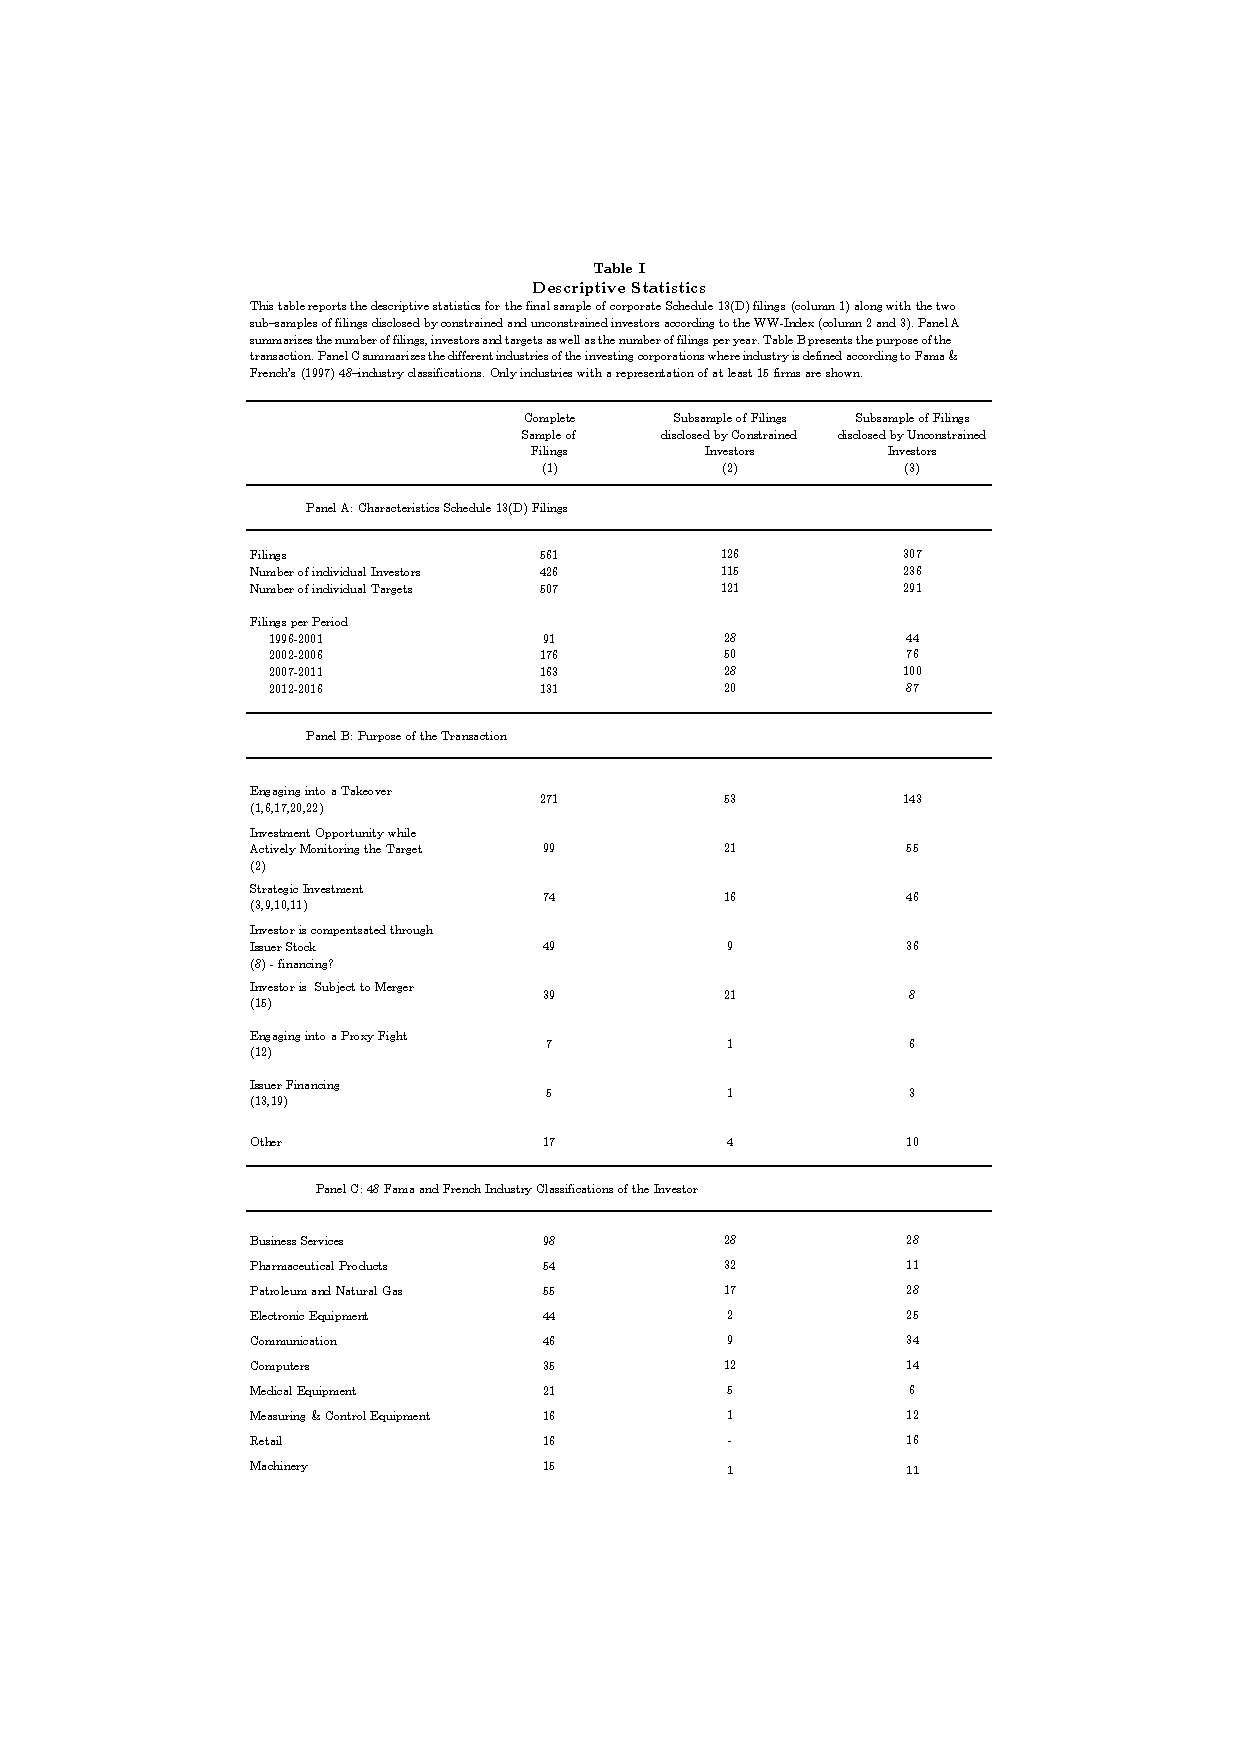
\includepdf[pages={1},pagecommand={},addtolist={1,table,Descriptive Statistics,descriptive}]{Descriptive_copy.pdf}

\begin{figure}[!htb]
	\centering
	\begin{adjustbox}{width=\textwidth}
		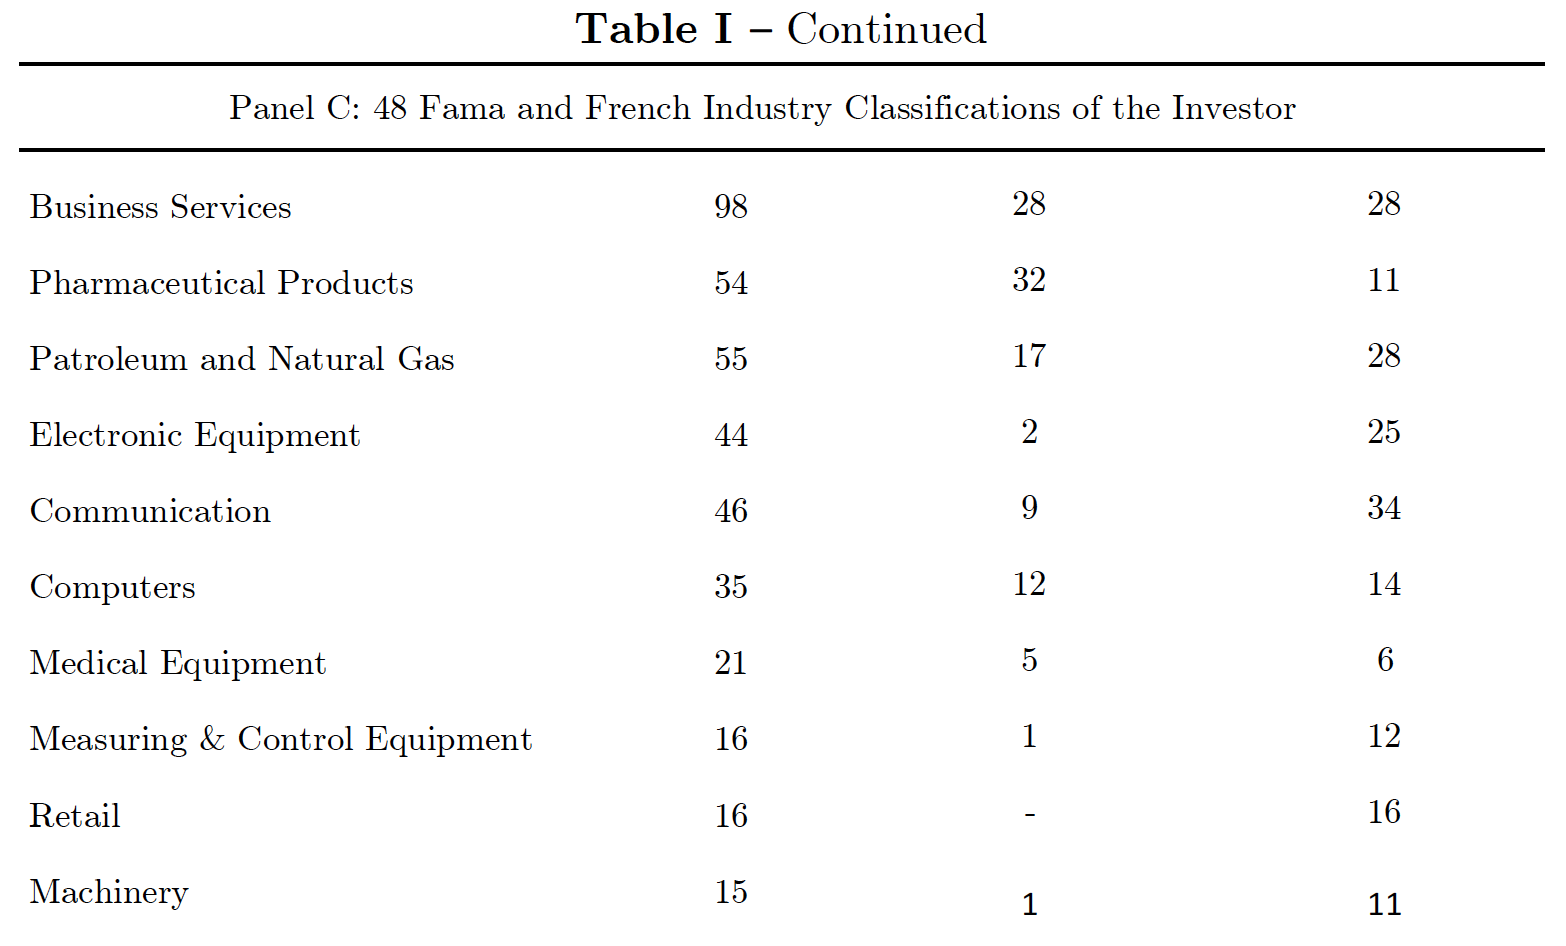
\includegraphics{Descriptive}
	\end{adjustbox}
\end{figure}
\noindent Panel B lists the extracted "Purpose of Transaction", which represents item 4 in Schedule 13(D) filings. The purpose is only explicitly stated if it occurrs in at least five filings. Furthermore, the two purposes \emph{Engaging into a Takeover} and \emph{Strategic Investment} group several purposes by common characteristics. According to \citet[p.1]{Betton2008}, filings disclosed with the purpose of a merger agreement, tender offer or hostile bid are grouped under the purpose \emph{Engaging into a Takeover} and filings disclosed due to alliance agreements, license agreements, strategic acquisitions and joint ventures are grouped under the purpose \emph{Strategic Investment}. A detailed description on how the filings were categorized can be found in Appendix B. 
Close to half of the investments were made while engaging into a takeover process and only 53 of these 271 filings were disclosed by constrained investors.\\
On the other hand, more than 50\% of the filings in which the investor was subject to a merger were disclosed by constrained investors -- the securities underlying the Schedule 13(D) were acquired to distribute them to own shareholders at the execution of the merger. In this scenario, the relationship between investor and target is switched.\\
With 99 filings, the second most reported purpose was essentially to invest in the target. The target is considered to be a good investment opportunity, frequently undervalued and the investing corporation aims actively monitor and interact with it. The main idea is these filings do not directly imply future collaboration but give room for speculations.\\
Following actively held investments, strategic investments are the third most common purposes due to which filings were disclosed. Different to the former, they are based on the premise of future collaboration between investor and target and thus denote a likely value improvement for the target. Potentially of high interest, they represent around one quarter of filings. Interestingly, 54 of all filings were disclosed due to investments for financing the issuer -- for instance direct financing or asset purchase agreements. This is in line with the findings of \citet[p.2792]{Allen2000} and \citet[p.78]{Liao2014} who suggest a driver of minority acquisitions is the target's financing. There are only 7 filings in which the investor announced a proxy fight with the target's management. In general, these findings are in line with the research findings on why corporation would actively hold equity ownership, namely in the process of takeover discussions, while building strategic alliances, for direct issuer financing or overcoming informational barriers.
Turning to Panel C, the major industries in which the investors operate according to their Fama \& French's 48 industry classification code are presented.\footnote{For simplicity, the SIC-Industry codes are not shown next to the Fama \& French industry classifications as these industries are compiled by several 3-digit SIC industries.} Shown are only industries, which are represented by at least 15 corporate investors. For the complete sample, 42 out of the maximum 48 industries are existent. As mentioned previously, the sample is reduced by excluding the trading industry due the irregular investment behavior. The highest industry representation is in business services with 98 filings, followed by the industries of pharmaceutical products, petroleum and natural gas and electronic equipment. For the business industry, equally 28 are investors constrained and unconstrained. Looking at pharmaceutical products, there are more constrained than unconstrained investors and their representation in the computer industry is almost the same. This could mean that especially in industries in which property rights become blurry and contracting is complicated hence information asymmetry is large, financially constrained firms have a higher representation \citep[p.4]{Liao2014}.
\begin{comment}
	\subsection{Examples of Corporate Activism}
	In this subsection, two cases of corporate investments into other firms are being described. The first example is takeover the second is strategic investment. 

	\subsubsection{Pfizer Inc. and Icagen Inc. }
	On June 24, 2011 Pfizer filed a Schedule 13(D) in which it declared an ownership of 14.2\% in Icagen Inc.. Pfizer was initially engaging with Icagen in accordance to a "collaboration agreement" dated August 13, 2007. In the purpose statement of June 24, 2011 Pfizer wrote: 
	\begin{center}
		"Pfizer is evaluating the possibility of entering into a strategic transaction with Icagen, which could have the effect of influencing or changing the control of Icagen by means of stock or asset acquisition or merger"
	\end{center}
	Consequently, the filing can be considered as firms strategic investment and the purpose statement can be classified as indicating that Pfizer wants to further strategically invest in Icagen.
	The ownership of 14.2\% in Icagen was acquired between 2007 and 2008. The collaboration agreement on August 13, 2007 involved the "discovery, development, manufacture \& commercialization of pharmaceutical compounds and products that modulate three specific sodium ion channels as potential new treatments for pain and related disorders". The investment resulted in Pfizer appointing the treasurer and president of Icagen as their proxies. 
	In order to extend the collaboration agreement, on September 17 2009 Pfizer and Icagen entered into the first amendment to the agreement. 
	On September 21, 2010, one year later, they entered into a second amendment to the collaboration agreement which would extend it until December 31, 2011. In the course of a further collaboration between Pfizer and Icagen after the expiration of the collaboration agreement , Pfizer filed this Schedule as stated in the purpose statement above.
	\pagebreak	
\end{comment}

\subsection{Identifying the Investors prior to their Schedule 13(D) Filing}

After being familiar with general characteristics of the sample's filings, this section focuses on identifying the corporations prior to their Schedule 13(D) filing. What type of corporation makes activist investments and what are the characteristics of firms identified to be financially constrained? Do all these measures overall identify similar investors?\\
Following, Table 2 introduces financial characteristics of each measure's sub-samples.\footnote{Note that investors are classified into three groups based on the tertile values of the financial constraint indices but only the top and bottom groups are presented. There exists a "gray zone" in which investors are not directly classified.} By the virtue of each measure, the two samples do not necessarily have to add up to the total number of filings. Hence for the WW-Index, the two sub-samples consist out of 307 and 107 investors. By grouping the investors according to their dividend pay out ratio, 184 investors are identified to be financially constrained and 310 as not. The HP-Index identifies only 58 constrained investors in the initial sample and only for the rating measure do the two groups include all investors with 296 having a credit rating and 265 missing one.\\
For each sample, Table 2 reports the mean [median] of several key financials. For the complete sample, standard deviation and both, lowest and highest value are shown additionally. Column (1) and (2) present financials of the two sub-samples identified by each measure, where constrained investors are in Column (1) and unconstrained in Column (2). Column (3) shows the $t$-statistic and $Z$-statistic for differences between financially constrained and unconstrained investor's means and medians. For all tests, the $t$-statistics are for differences in means, assuming unequal variances between the two samples. The null hypothesis to be tested is that the population means from the sample of constrained and unconstrained investors are equal $H_{0}: \mu_{1}=\mu_{2}$. The two-sided alternative hypothesis reads $H_{a}: \mu_{1}\neq\mu_{2}$, thus both means are unequal and there exists a difference.\footnote{assumptions?} In addition to the parametric $t$-statistic, the non-parametric Wilcoxon Mann-Whitney $Z$-statistics tests similar to \citet[p.201]{Klein2009} whether the samples of constrained and unconstrained investors are from populations with the same distributions. It can also be called a test of differences in the medians, if the two sample distributions have the same shape. The data analysis is conducted by using the statistical program Stata (Version 13.2, StataCorp, College Station, Texas). Specifically, the Mann-Whitney test is conducted by using the command -ranksum- based on \citet[p.59]{Mann1947}. All reported data corresponds to the investor's fiscal year which is closest to the filing date and the reported values are winsorized at the 1\% and 99\% levels so that extreme values are replaced by the respective percentiles. This enables a presentation of more meaningful mean statistics \citep[p.203]{Klein2009}. 
\pagebreak

\begin{sidewaystable}[!htbp]
	\centering
	\captionsetup{textformat=empty,labelformat=blank}
	\caption{Characteristics of Investors prior to their Schedule 13(D) Filing}
	\textbf{Table II}\par\medskip
	\large\textbf{Characteristics of Investors prior to their Schedule 13(D) Filing\\}\par\medskip
	\justifying
	\footnotesize\noindent\setstretch{1.2}This table summarizes characteristics of the investors for the complete sample, and the sub-samples of each measure of investor's financial constraints (column 1 and 2). For the complete sample,  standard deviation and minimum and maximum value of the variables are shown. For each variable, the mean [median] is reported. All data are winsorized at the 1\% and 99\% levels. Column (3) of each measure shows the t-statistic [Z-statistic] testing for differences between financially constrained and unconstrained investors means [medians]. All accounting data are from the end of the fiscal year preceding the Schedule 13(D) filing date reported by the SEC. Panel A presents measures of the investor's profitability, Panel B displays  measures of cash balances and debt and Panel C gives information on the investor's size and Investment. See Appendix A for variable definitions. ***significant at the 0.01 level; **significant at the 0.05 level; * significant at the 0.10 level.\par\medskip
	\centering													
	\begin{adjustbox}{width=\textwidth}
		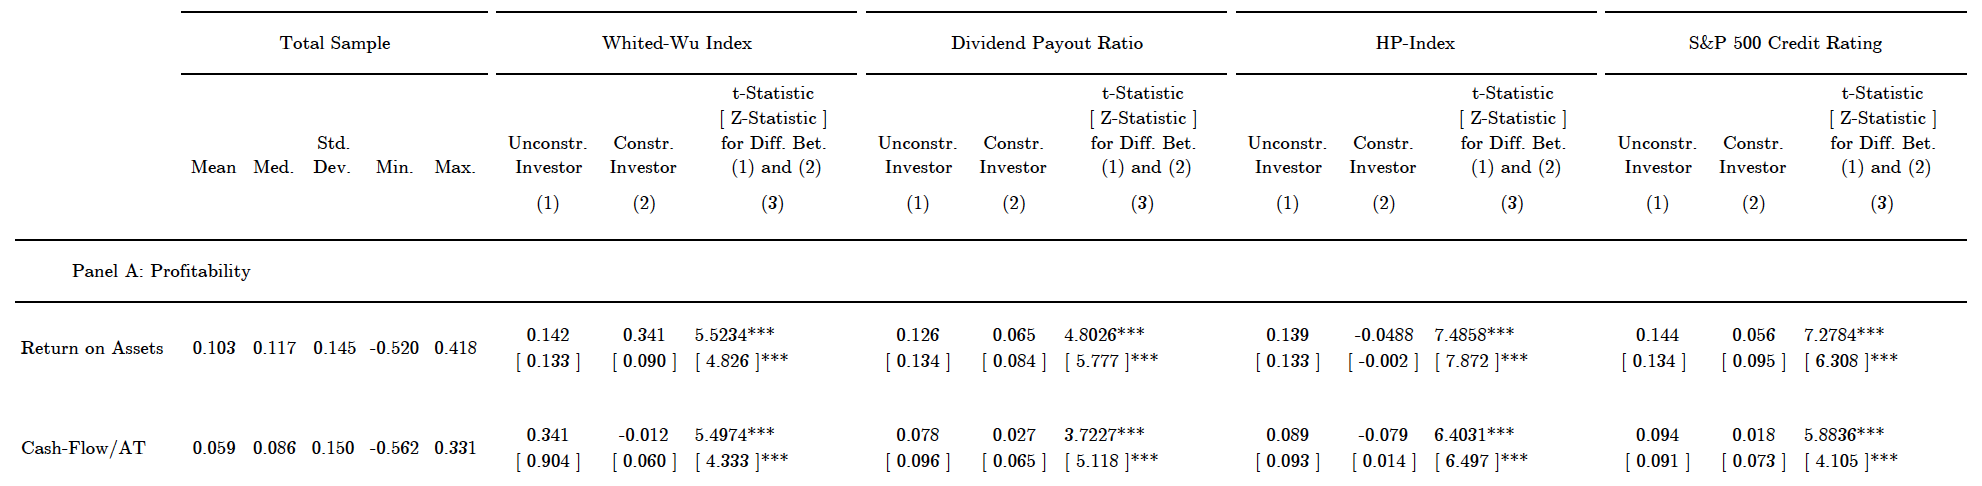
\includegraphics{Summary1}
	\end{adjustbox}\par\medskip
\end{sidewaystable}

\begin{sidewaystable}[!htbp]
	\centering
	\begin{adjustbox}{width=\textwidth}
		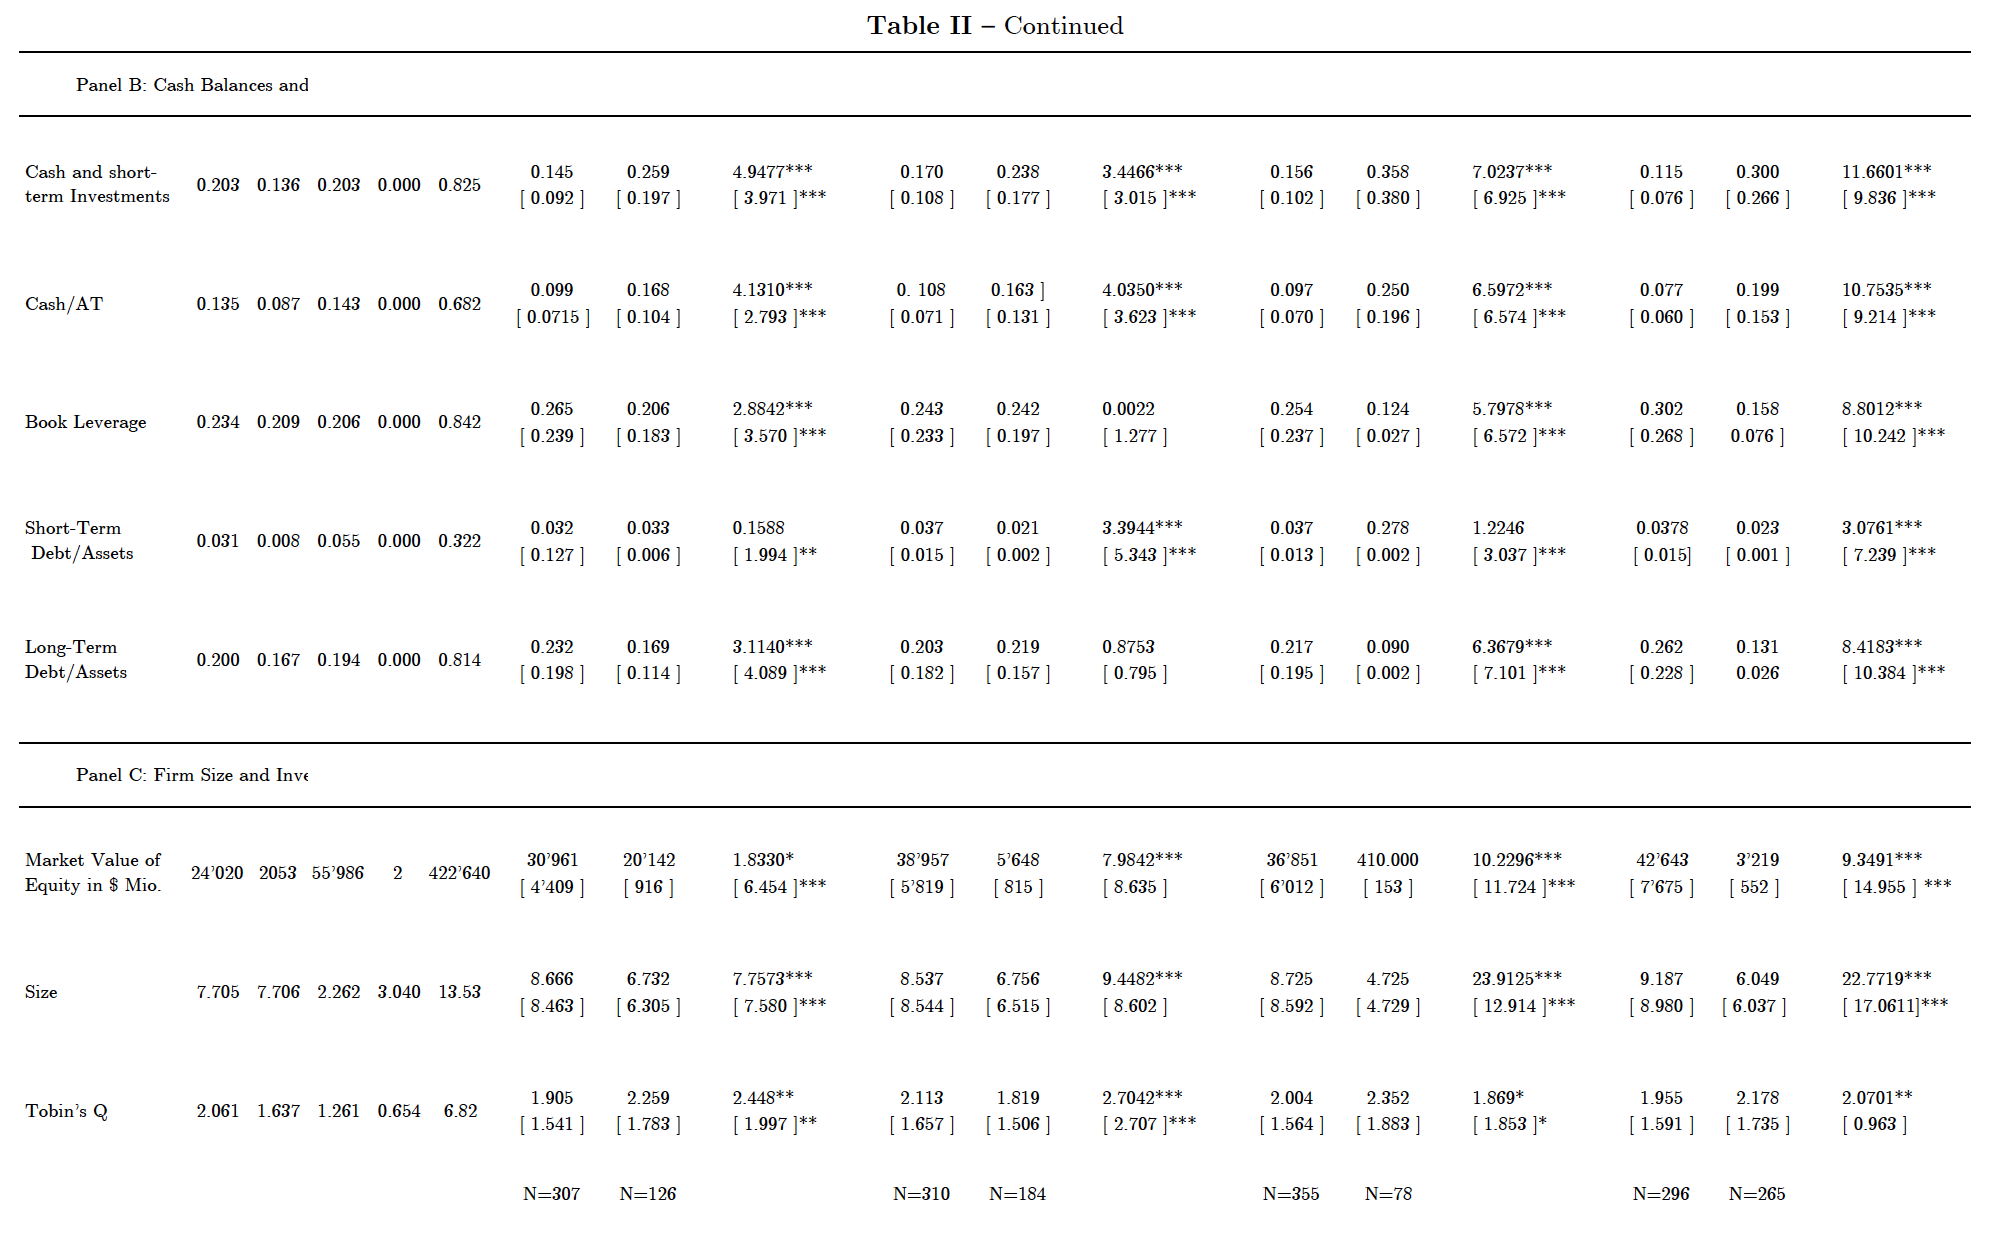
\includegraphics{Summary}
	\end{adjustbox}
\end{sidewaystable}

\pagebreak
\noindent Moreover, characteristics for the WW-, HP- and Dividend Payout indices have explanatory power beyond the sample, as these investors are identified according to their comparative values across the entire Compustat database. 
%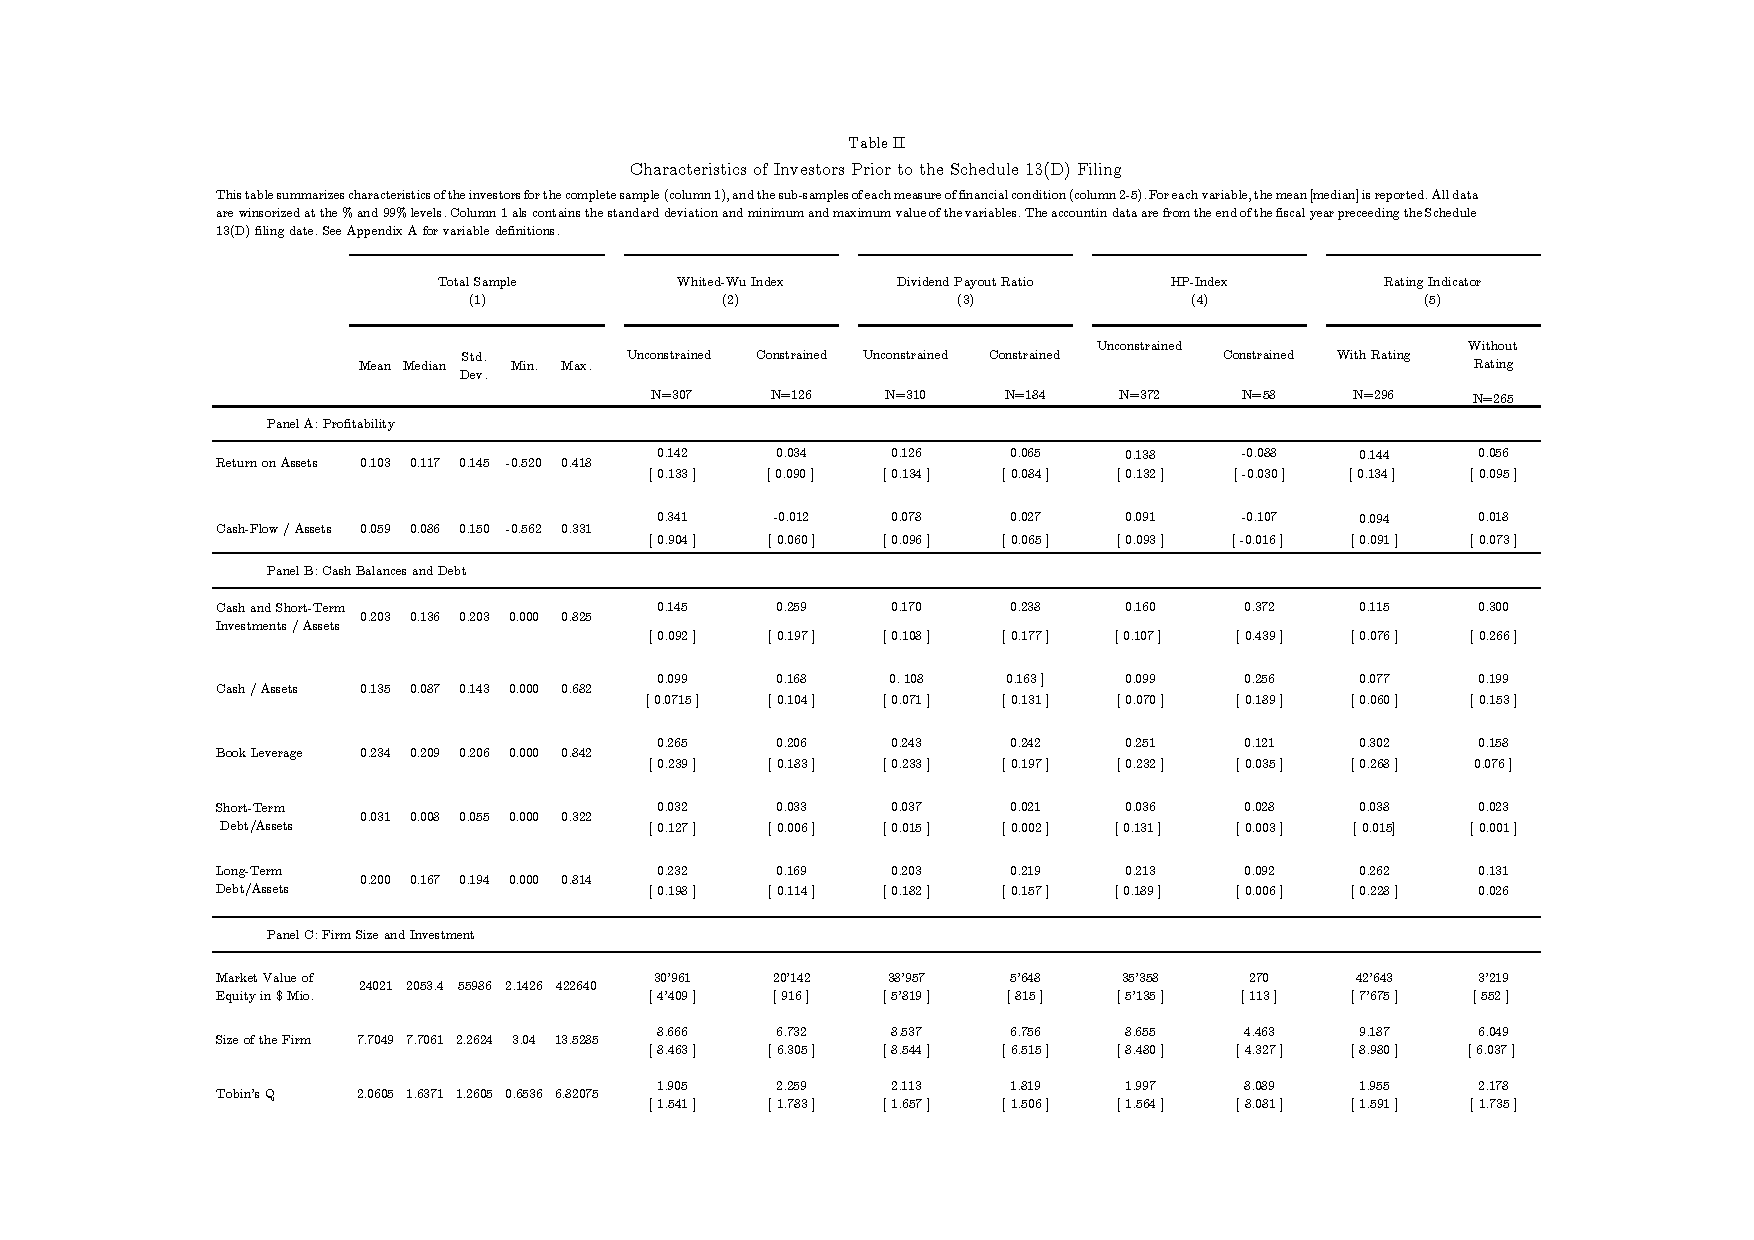
\includepdf[angle={90},pages={1},pagecommand={},addtolist={1,table,Characteristics of Investors prior to their Schedule 13(D) Filing,Summary}]{Summary_copy.pdf}
Hence, a loose comparison to samples of other studies is possible. For further simplicity, the notion of "financially constrained" is used independently of the measure initially used to identify them. \\
% For all following tests, the $t$-statistics are for difference in means, assuming unequal variances between the samples. The $Z$-statistic is a Mann-Whitney rank-sum test for equality of medians on unmatched data and 
Panel A reports two ratios on profitability -- return on assets (ROA), defined as earnings before interest and taxes (EBITDA) to total assets and the ratio of cash flow from operations to total assets. On average, the sample's corporations have positive returns and a fairly small 0.059 cash flow ratio. Across all measures, financially constrained investors have a ROA which is significantly lower when compared to their counter-samples. Turning to the HP-Index, for financially constrained investors the return from the fiscal year prior to the filing is even negative. Furthermore, investors in this group also have a negative cash flow (same for the Whited-Wu index) and again, the difference between constrained and unconstrained investors is apparent across all measures. This implies that in general, constrained investors seem to be less profitable \citet[p.544]{Whited2006}. \\
Panel B reports ratios on cash balances and debt. Constrained firms have considerably larger amounts of cash reserves (both cash and short-term investments) reflecting their dependency on internal funds when it comes to investments \citep[p.142]{Fazzari1988}. Unsurprisingly, book leverage, defined as long-term debt plus current debt to total assets \citep[p.1440]{MacKay2005} is higher for firms considered to be financially unconstrained, as financially constrained firms face the issue of restricted access to external finance. Across all sub-samples, the ratio of short-term debt to total assets is fairly small and only marginal differences exist. These characteristics show sub-samples similar to those presented in \citet[p.544]{Whited2006} and \citet[p.1917]{hadlock2010} and thereby suggesting a successful implementation of the measures on the initial sample of Schedule 13(D) filings.

Facing Panel C, information on firm size and investment is presented. The market value of equity is defined as the closing price at the end of the fiscal year times the number of shares outstanding. Through all measures, financially constrained firms have a lower market value of equity when compared to their counter samples. The largest difference is among the two samples classified by the HP-Index. This however is unsurprising, as it only includes the two variables size and age and with size playing a determining role. Similar differences are apparent in the variable size, defined as the natural logarithm of total assets. In conclusion, this suggests the variable size (or market value) is an important determinant across all measures. Lastly, Panel C presents the investors investment opportunity in the form of Tobin's Q \citep[p.1441]{MacKay2005}, which is measured according to \citet[p.1]{Khatami2014}. Constrained firms have a higher Tobin's Q which may be evidence of their unexploited investment opportunities \citep[p.539]{Whited2006}. This attribute holds for all sub-samples, except for the two identified by the investor's dividend payout ratio. 


To conclude, firms identified to be constrained in the sample of corporate activist investors are less profitable, hoard more cash and have less debt when compared to unconstrained firms. They are usually smaller in size and have more unexploited investment opportunities. Across all measures, financial characteristics tend to move in the same direction and they show similarities to those of other studies (see \citet[p.544]{Whited2006} and \citet[p.1917]{hadlock2010})

\section{Market Reactions to 13(D) Filings -- Abnormal Stock Returns}
% Intention
In analyzing whether the financial condition of the activist corporate investor matters, abnormal share price reactions around the filing date identify the effect the 13(D) filing has on the target's stock, likewise the market's perception of value improvement, after accounting for general market movements.
The set up of the event study performed for this purpose is as follows: The time line consists successively of the estimation window, in which parameter estimates are obtained, the event window for which the abnormal returns are computed and the post event window. 
The filing date, as reported by the SEC and reported on EDGAR is set as the event day. For simplicity, the event window [x,y] is determined relative to the event day 0 with x days before and y days after the filing date. Abnormal returns are computed for various event windows. For that reason, the estimation window is set 120 days prior to the largest event window. With the largest event window starting 30 days before the event day, the estimation window begins 150 days prior to the actual event day.\\
The abnormal return $AR_{i,t}$ for the target's security $i$ at day $t$ is defined as the difference between the actual (observed) return $R_{i,t}$ and the expected return $E(R_{i,t}|X{t})$ given the absence of the event \citep[p.15]{MacKinlay1997}:
	\begin{equation}\label{eq:1}
		AR_{i,t}=R_{i,t}-E(R_{i,t}|X_{t})
	\end{equation}
The expected return $E(R_{i,t}|X{t})$ is the result of an estimation based the market model, in which the value-weighted NYSE/Amex/Nasdaq index from CRSP proxies for the market return $R_{M,t}$ and likewise is the independent variable \citep[p.18]{MacKinlay1997}.
	\footnote{For the expected return the market model assumes a constant and linear relation between the observed returns $R_{i,t}$ and the return of a market index $R_{m,t}$ \citep[p.18]{MacKinlay1997}. The parameters are estimated by ordinary least squares regressions based on estimation-window observations of stock returns.}
This yields the abnormal return $AR_{i,t}$
	\begin{equation}\label{eq:2}
		AR_{i,t}=R_{i,t}-(\hat{\alpha_{i}}+\hat{\beta_{i}}R_{M,t})
	\end{equation}
To accommodate for a multiple period event window and to draw overall inferences of the Schedule 13(D) filings \citep[p.21]{MacKinlay1997}, the abnormal returns $AR_{i,t}$ for target $i$ are aggregated over the event window $(\tau_1,\tau_2)$. 

For robustness, two different methods in aggregation over time are used. The cumulative abnormal return $CAR_{i,(\tau_1,\tau_2)}$ and the abnormal buy-and-hold return $BHAR_{i,(\tau_1,\tau_2)}$.\\
The cumulative abnormal return $CAR_{i,(\tau_1,\tau_2)}$ for security $i$ in event window $(\tau_1,\tau_2)$, is the sum of the abnormal returns $AR_{i,t}$ from equation \eqref{eq:2}.
	\begin{equation}
		CAR_{i,(\tau_1,\tau_2)}=\sum_{t=1}^{T}AR_{i,t}
	\end{equation}
The second method of aggregation over time is the abnormal buy-and-hold return $BHAR_{i,(\tau_1,\tau_2)}$. It is independent from the results of equation \eqref{eq:2} and no estimation window is required. 
The abnormal buy-and-hold returns $BHAR_{i,(\tau_1,\tau_2)}$ are the difference between the realized (observed) buy-and-hold returns and the normal buy-and-hold returns $R(R_{i,t}|X_{t})$.
But in contrast to the cumulative abnormal return, the buy-and-hold return mimics the investment strategy of investors that buy the stock and hold it for a longer period of time. In this sense, the actual (normal) buy-and-hold return on day $t$ is the return on day $t$ times its lagged return on day $t_{-1}$. This means that for the target's security $i$ in the event window $(\tau_1,\tau_2)$ the abnormal buy-and-hold return $BHAR_{i,(\tau_1,\tau_2)}$ is
\begin{equation}
	BHAR_{i,(\tau_1,\tau_2)}=\prod_{t=\tau_1}^{\tau_2}(1+R_{i,t})-\prod_{t=\tau_1}^{\tau_2}(E(R_{i,t}|X_{t})
\end{equation}
Analogous to the estimation of normal returns for equation \eqref{eq:2}, the value-weighted NYSE/Amex/ Nasdaq index from CRSP is used to calculate the normal buy-and-hold returns in the respective event windows $(\tau_1,\tau_2)$ \citep[p.25]{Brav2009}.

\subsection{Time Series of Abnormal Returns}

Graph 1 plots the times series of average cumulative abnormal returns for securities subject to all filings and subject to filings of constrained and unconstrained corporate investors (grouped by the WW-Index). This means, average abnormal returns are calculated by grouping targets based on characteristics of the investor. A first glance reveals that independent of the investor, all three lines evolve almost equally until day -10. In the following days, targets of financially constrained investors experience smaller abnormal returns, that is their aggregation continues to proceed below the other two. Considering the fact they peak at around 8\%, targets of unconstrained investors experience cumulative abnormal returns considerably higher with close to 20\%. In-between, abnormal returns for the complete sample of targets aggregate to approximately 15\% during the 41-day window. This is approximately 5\% more compared to the 10\% reported in \citet[p.1563]{Collin-Dufresne2015}. 
Figure 1 indicates that abnormal returns for targets of financially constrained investors differ in magnitude and thus presents first evidence that financial constraints of corporate activist investors could matter to the market.


\begin{figure}[!htb]
	\centering
	\captionsetup{textformat=empty,labelformat=blank}
	\caption{Time Series of Cumulative Abnormal Returns}
	\begin{adjustbox}{width=\textwidth}
		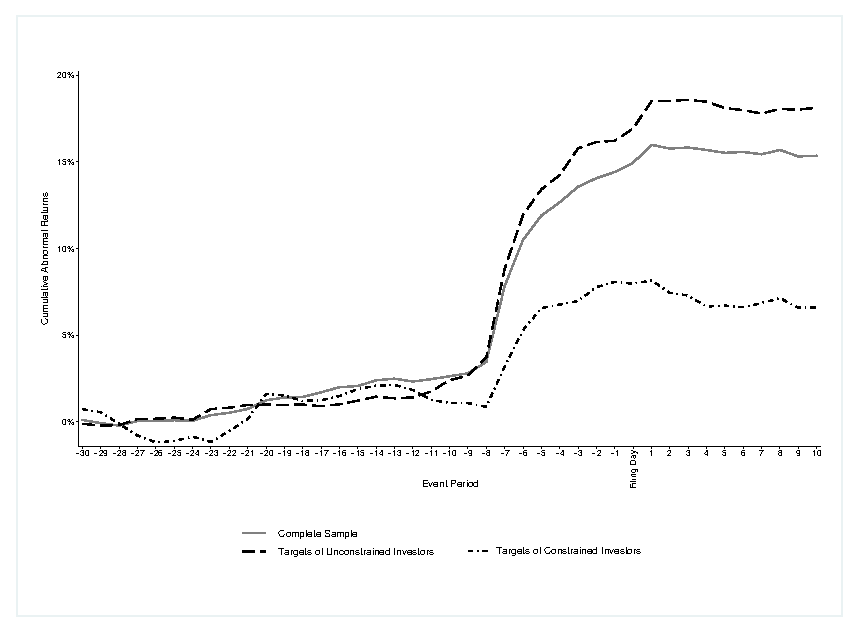
\includegraphics{WW-TimeS_copy.eps} \label{AR}
	\end{adjustbox}
	\justifying
	\noindent\footnotesize\setstretch{1.2}\textbf{Figure 1. Time Series of Cumulative Abnormal Returns.} The solid line plots the time series of average cumulative abnormal returns for all targets where the cumulative abnormal returns is the aggregation of abnormal returns up to each point in time using the market model with the value-weighted NYSE/AMEX/Nasdaq index from CRSP as the market return from 30 days prior to the filing date to 10 days afterwards. Equivalently, the dashed (dashed-dot) line plots the average cumulative abnormal returns for targets of financially unconstrained (constrained) investors. \par\medskip
\end{figure}
Furthermore, Figure 1 reveals that in all three cases, abnormal returns start to occur extensively in the [-11,-8] period, implying that valuable information -- in any form -- is available before the actual filing. Although the behavior is in line with that presented in \citet[p.1563]{Collin-Dufresne2015}, \citet[p.370]{Greenwood2009} and \citet[p.1756]{Brav2008}, possible explanations are the following: Stock market participants might knew about the pending stake before it was announced, for which \citet[p.2802]{Allen2000} choose their event window to be [-10,10]. This is equivalent to information leakage for which \citet[p.31]{Brigida2012} find evidence prior to the actual filing date. Furthermore, filings may not be reported until several days after the actual investment for which reason \citet[p.87]{Liao2014} also implements a longer event window.
These possibilities are in line with general characteristics of Schedule 13(D) filings, as Section 13(d) grants the investor a 10-day window after passing the 5\% threshold for disclosing the filing. 
As it is the investor's own actions that potentially increase the value of the target firm, a potential increase in their trading activity could also explain the early upsurge. This approach is adopted from  \citet[p.1561]{Collin-Dufresne2015} who analyze the trading strategy of informed Schedule 13(D) filers. Firstly, they find that trading activity increases in the [-12,-9] period in which the reported event dates are clustered (date on which the 5\% threshold is passed). Secondly, they show that close to 1\% of outstanding shares are purchased on the event date, compared to only 0.10\% and 0.15\% on the days before and after the event date \citep[p.1561]{Collin-Dufresne2015}. Thirdly they note that the prices move up when Schedule 13(D) filers trade. By combining these three findings, an explanation could be that by their own trading at the event day, corporations drive up prices. This argument however is limited, as constrained firms experience small negative abnormal returns in this period. Summarizing these explanations, \citet[p.207]{Klein2009} start their event window at day -30 to allow for the 10-day 13(D) filing window, possible prior leakage of information and prefiling price pressure.\\
That is to say, these researchers have expanded their event-windows to overcome the difficulty of identifying the precise date on which the information reaches the market. This adjustment might create problems as the number of confounding events increases \citep[p.352]{mcwilliams1999}. For that reason, the sample of Schedule 13(D) filings was cross-referenced with a sample of activism filings provided by SharkRepellent. This however lead to only 40 matched campaigns occurring in the same month of each target's Schedule 13(D) filing. For these 40 matches, the reported announcement date by SharkRepellent was either equal to or later than the reported filing date of the respective Schedule 13(D) and thereby revealing no additional information on the Schedule 13(D) filings.

% So in the window [-10,0] other public announcements corresponding with the investment can be made. If for example a takeover announcement is made public during the ten days in which the firm is not obligated to file, the abnormal returns might be due to the takeover announcement. This means, the filing itself has little impact and is just a necessary accompaniment.  With regards to the remaining purposes of transaction, there is no reason to believe they follow a similar pattern. 
% A scenario in which a different announcement triggers the abnormal share price reaction is conceivable. So when assessing the true impact of the filing, all abnormal returns in the event-window [-10,0] should be neglected and only those occurring after the announcement, including the event day, should be utilized. This however is a limited approach, as the announcement still affects the abnormal returns in the event window of the filing and a strict separation over time would not mitigate all the announcement effects.\\
% In an attempt to isolate possible effects of takeover announcements on abnormal returns around day -7, a second graph excluding takeover filings was plotted. The graph showed that abnormal returns primarily decrease in magnitude and that the early impact on the target's stock remained at around day -7. This means that even when controlling for the largest sub-sample which simultaneously is the only one for which an earlier announcement is plausible, the early impact is still existing. The reduction in abnormal returns however implies, that large chunks are driven by filings with the purpose of a takeover. 
\subsection{Event Windows and Financial Constraints}

For the aforementioned reason, Table III present the mean [median] cumulative and buy-and-hold abnormal returns for the following four event windows: Event window 1 is [-10,3], to allow for the 10-day filing window, information leakage and accommodate subsequent press coverage. The second event window is [-10,-6] to detach the possible effect of information leakages and event-date trading. Analogous, the third event window [-5,3] aims to control for these two. This seems to be reasonable, as the aggregation of abnormal returns in Graph 1 slows down at around day -5, implying that information has been processed. The fourth event window is [-1,3] to accommodate for just the filing date and press coverage.
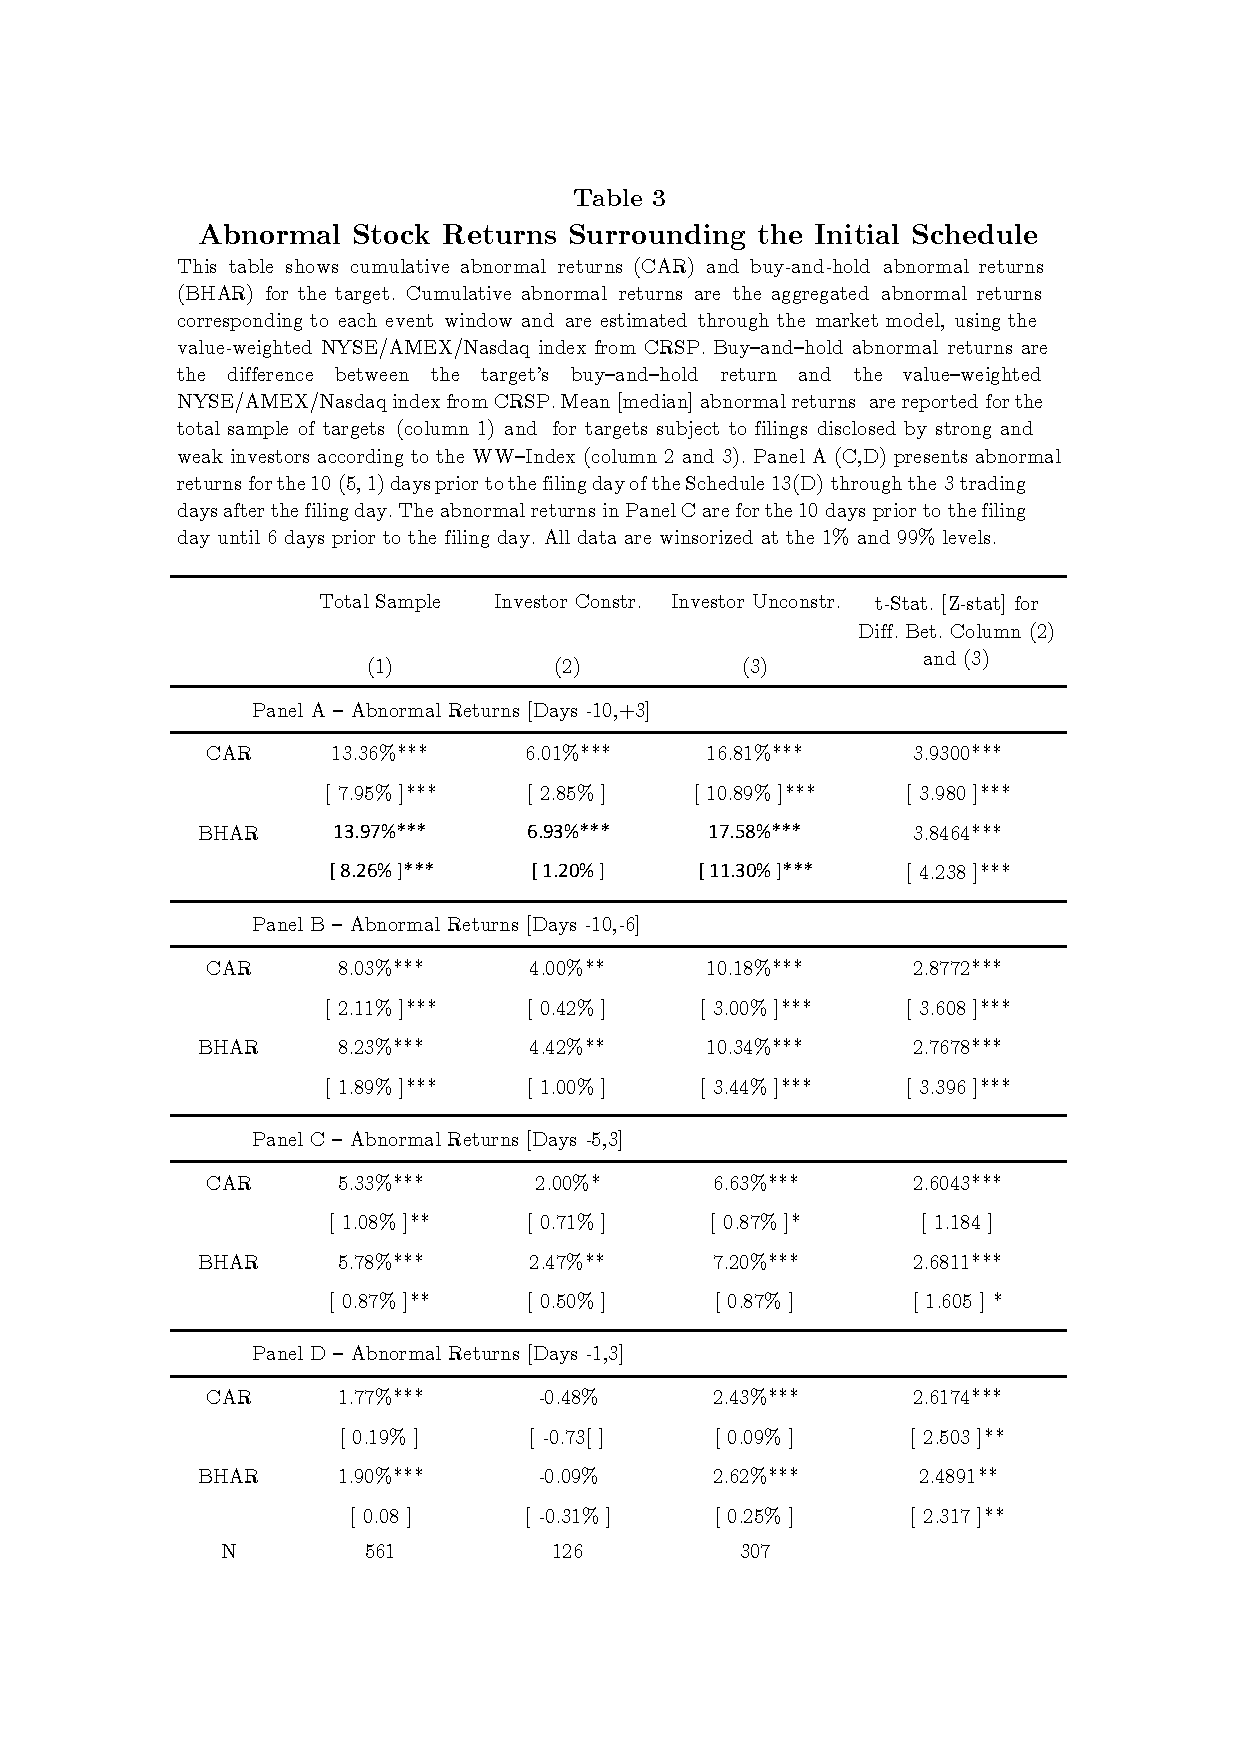
\includepdf[pages={1},pagecommand={},addtolist={1,table,Abnormal Stock Returns Surrounding the Initial Schedule 13(D) Filing,windows}]{AR_by_Window_copy.pdf}

\noindent Column (1) presents the abnormal returns for all targets. Column (2) and (3) show the abnormal returns for targets dependent on their investor's financial condition. The investors are grouped by the Whited-Wu index and groups are equal to those presented in Table II, with 126 filings disclosed by constrained and 307 disclosed by unconstrained investors.\\
For the abnormal returns in columns (1), (2) and (3), significance levels are shown. The null hypothesis to be tested is that the mean day abnormal return is equal to zero, and thus concerns the average effect of an event on returns to shareholders. If the average abnormal returns are independent, identical distributed, and normal, the test statistic is distributed Student-$t$ under the null hypothesis \citep[p.7]{Brown1985}. As shown in \citet[p.11]{Brown1985}, the $t$-Statistic can be applied even under the assumption of non-normality and a sufficient adjustment for cross sectional dependence is the application of the market model for estimating abnormal returns \citep[p.22]{Brown1985}. Therefore, the statistical significance of the cumulative abnormal returns is given by a two-tailed $t$-test for which the alternative hypothesis is defined as: cumulative abnormal returns are different from zero. The statistical significance of the median is computed by a quantile regression of the abnormal returns where the p-value of the coefficient represents the statistical significance of the median \citep{Ucla}. Column (4) tests the difference in means [medians] of column (2) and (3). As in Section 3, the $t$-statistics represents the standard parametric test for difference in means and $Z$-statistic is the non-parametric Mann-Whitney rank-sum test .
%\citet[p.15]{Brown1985} shows that results are not radically altered where there is clustering in event dates  and hence dependence of the excess return measures. 
%However, while extraction of the market factor via the market model appears to be a sufficient adjustment for dependence, this result is for randomly selected securities. \citep[p.22]{Brown1985}
All returns  presented in Table III are winsorized at the 1\% and 99\% level. This extensive presentation of abnormal returns is done for three reasons. Firstly, to check the differences in abnormal returns over varying event windows and thereby accomodate for the time-effect. Secondly, to check whether the estimated abnormal returns are similar for the two methods of measurement and thirdly to test whether the investor's financial condition matters independently of time (across all event windows).

Panel A presents the abnormal returns for the largest event window [-10+3]. Both, cumulative and buy-and-hold abnormal returns are positive and strongly significant at the 1\% level with mean abnormal returns being 13.36\% and 13.97\% respectively. Consistent with Graph 1, targets of unconstrained investors have a mean CAR and BHAR of 16.81\%, around 10\% higher when compared to those of constrained investors. For both, CAR and BHAR, the difference in abnormal returns across the two groups is statistically significant at the 1\% level. This shows, the investor's financial condition does matter economically and statistically when comparing the two means. These findings are supported by differences of around 7\% in medians. Furthermore, the abnormal returns of around 13\% are different to those observed in \citet[p.208]{Klein2009} but support \citet[p.29]{Brigida2012} findings that abnormal returns are higher for non-financial corporations.

Turning to panel B, the largest runup happens in the [-10,-6] event window. Abnormal returns aggregate to around 8\%, making up more than 50\% of the total [-10,3] runup. These results are matching with \citet[p.32]{Brigida2012} who find that the target's runup is greatest during the event window [-10,-6]. Again, targets of weak investors only gain 4\% whereas those of unconstrained investors have abnormal returns up to 10.30\%. Furthermore, the difference in means is is significant at the 1\% level for both methods of estimation.




% was will ich hier eigentlich sagen!! 
In Panel C, abnormal returns for the event window [-5,3] are shown. Independent of the investor, all targets experience a mean CAR of 6.63\%, significant at the 1\% level. Here too, targets of unconstrained investors outperform those of weak investors with around 5\%, while being statistically significant at the 1\% level.\\
Turning to abnormal returns for the smallest event window [-1,3] in Panel D, targets on avberage gain 1.77\% which is significant at the 1\% level. Hence a positive market reaction at the announcement of the filing exists and is not only apparent in the previous days. Striking is that on average, targets of constrained investors now experience negative returns although statistically not different from zero. Furthermore, the difference among the two samples is immensely high with approximately 3\%. Especially when considering the short event window and the already low-level of abnormal returns is the difference apparent.

Concluding, both buy-and-hold and cumulative abnormal returns show similar results with positive and significant market reactions in all event-windows surrounding the Schedule 13(D) filing date. Furthermore, the largest aggregation happens in the [-10,-6] event window but is not exceptionally high when compared to the overall runup. Most importantly however is the difference in abnormal returns for targets of financially constrained and unconstrained investors. The difference is present, both on an economic and statistical level. When testing the differences in means, it is significant across all event windows and thus independent from the time-effect. These findings present further evidence that the financial constraints could matter. 

\subsection{Financial Constraints and Purpose of Transaction}
So far it has been shown that independent from the event window, targets of financially unconstrained corporate investors gain on average significantly more, when compared to those of financially constrained investors. Attached thereto, this section aims to analyse whether this difference is existent across filings' different transaction purposes and across different measures of financial constraints.\\
For this reason, Table 3 presents the mean [median] cumulative abnormal returns from the [-10,+3] event window for each each measure and further for different transaction purposes. The measures of financial constraints and among which the sample separation takes place are the Whited-Wu Index, the investor's dividend payout ratio, the HP-Index and lastly the investor's S\&P's long-term issuer credit rating. For comparison, Panel A shows the abnormal returns for the complete sample of targets whereas Panel B presents the abnormal returns dependent on the filings purpose. Hence \emph{Engaging into a Takeover} involves merger agreements, tender offers and hostile bids and \emph{Strategic Investments} represents alliance agreements, license agreements, strategic acquisitions and joint ventures. \emph{Other Purposes} groups the abnormal returns for the remaining transaction purposes. For each measure, Column (1) and (2) present mean [median] cumulative abnormal returns for the two sub-samples. Column (3) tests the difference between column (1) and (2) and displays the  $t$-statistic [$Z$-Statistics].

Turning to Panel A, it presents the abnormal returns for all samples, without specifying the transaction the purpose. Across all measures, targets of financially constrained investors have significantly lower abnormal returns in the [-10,3] event window. Starting with the samples formed by the Whited-Wu index, the difference for the mean CAR is 10\% and significant at the 1\% level. Targets of unconstrained investors gain 16.81\% and those of constrained only 6\%. Similar conclusions can be drawn when comparing the samples grouped by the investor's dividend payout ratio. Targets of constrained investors encounter abnormal returns of 9.79\% compared to the 15.76\% for unconstrained investors. Again, the difference in means is significant at the 5\% level and comparing the sub-samples of the HP-index yields similar results -- targets of constrained investors experience abnormal returns of 9.18\%, those of financially unconstrained investors 16.2\% and the 7\% difference in means is significant at the 5\% level. On the other hand, the difference in market reactions to filings of investors with and without a credit rating is present but has no statistical significance. An explanation could be a possible upward bias in mean abnormal returns for the sample of constrained investors, as some of the least constrained corporations might lack a credit rating and are therefore mistakenly identified as financially constrained \citep[p.18]{heller2015}.
Nonetheless, across all measures is a difference in the mean cumulative abnormal returns visible, further indicating that financial constraints might  matter when the market assesses the value improvement for the target.   
%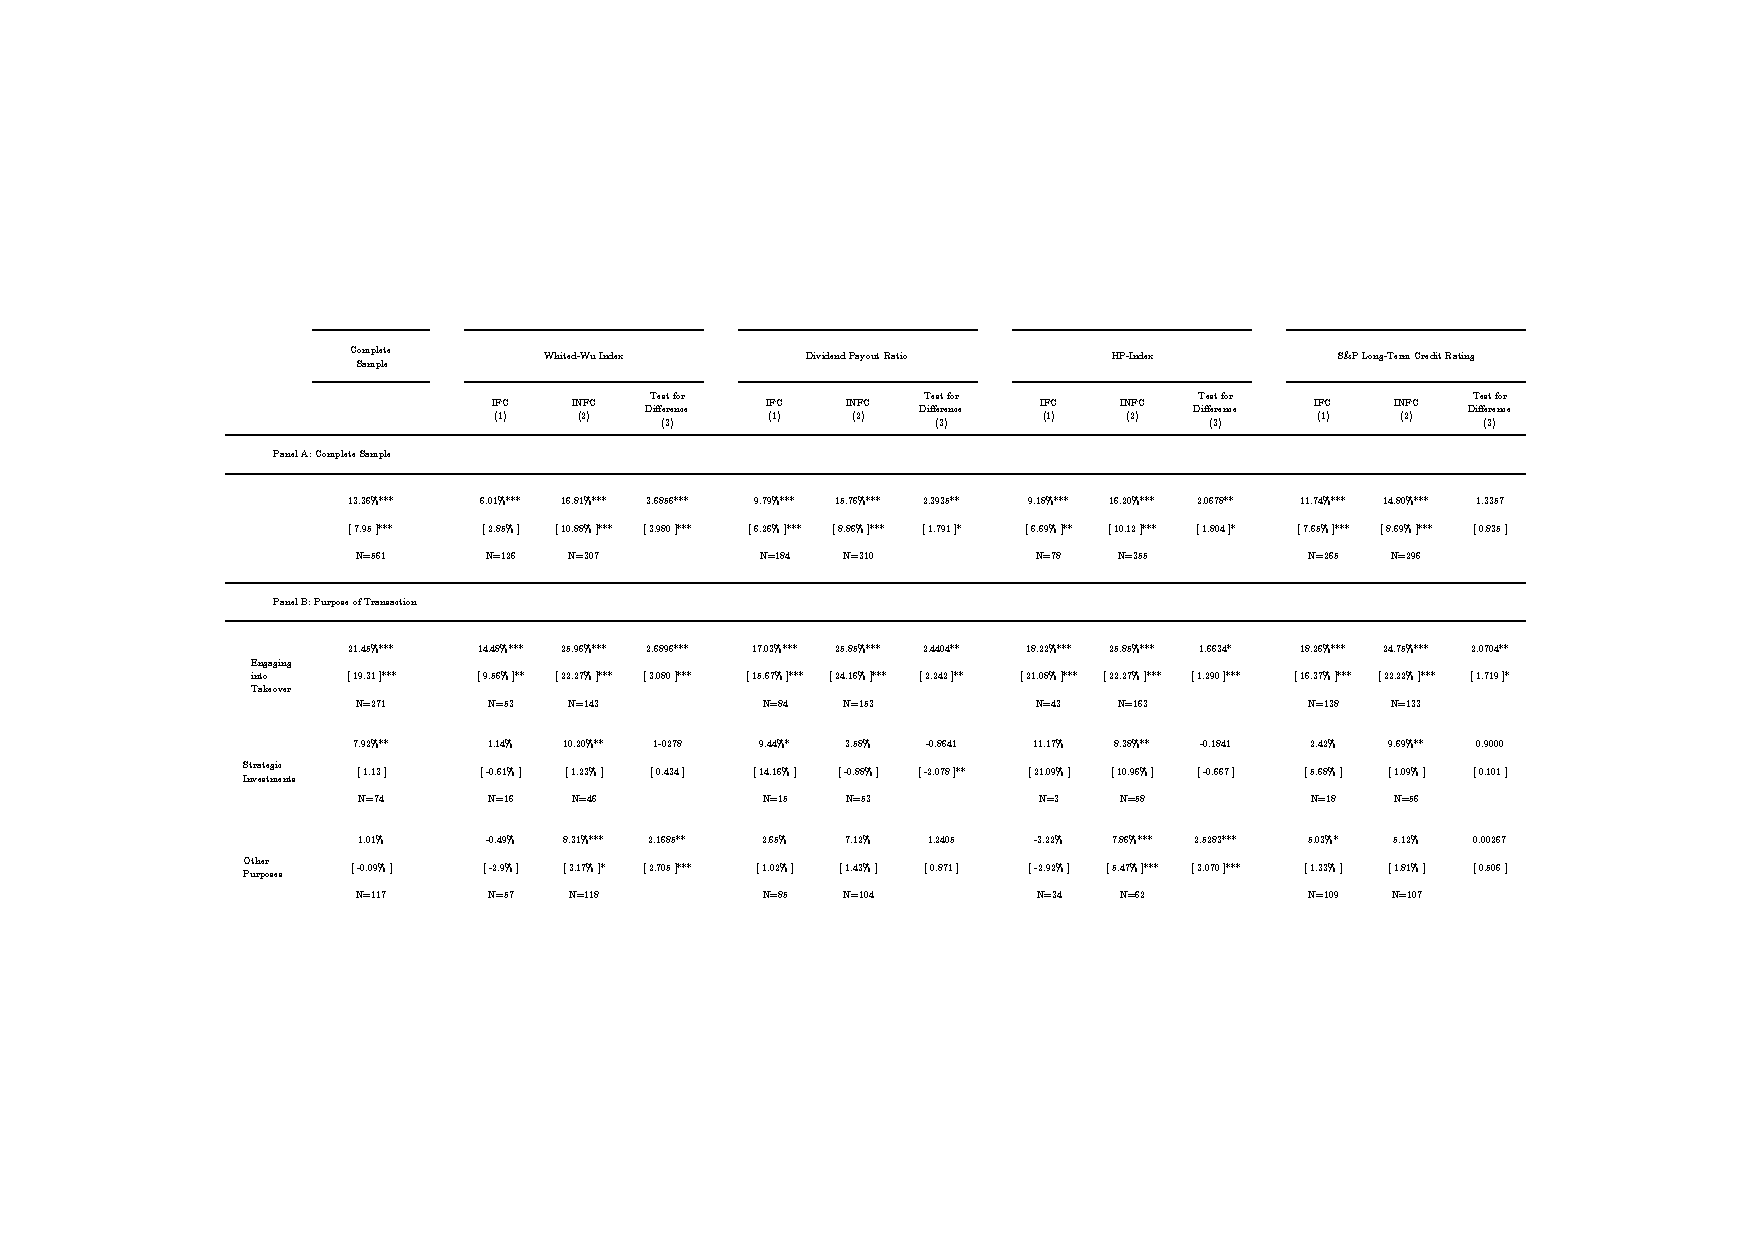
\includepdf[pages={1},pagecommand={},addtolist={1,table,Abnormal Returns by Measures of Financial Constraints and Purpose of Transaction,measures}]{Ar_by_Measure_copy.pdf}
Facing Panel B, abnormal returns of targets are now additionally sorted by the filing's purpose of transaction. The purpose of engaging into a takeover generates the strongest market reaction with a mean CAR of 21.45\% for the 271 targets and cross all measures, targets of financially unconstrained investors have a CAR of roughly 25\% for the [-10,3] event window. \citet[p.112]{Khatami2014} have similar results for acquisition announcement returns when the acquirer is financially unconstrained with an 11-day CAR of 25\%. The difference in abnormal returns is the largest for the Whited-Wu index and the smallest for the investor's credit rating which is analogous to Panel A. For all measures, except the HP-index, the difference in mean CAR's is significant at least at the 5\% level. For targets of investors grouped by the HP-Index, the difference is only significant at the 10\% level which might be due to the its low sample size of only 43 filings from constrained investors. Nonetheless, the univariate comparison reveals that investors' financial constraints might be especially important in the context of mergers and acquisitions \citep[p.112]{Khatami2014}.

\begin{table}[!htbp]
	\centering
	\captionsetup{textformat=empty,labelformat=blank}
	\caption{Abnormal Returns by Measures of Financial Constraints and Purpose of Transaction}
	\textbf{Table IV}\par\medskip
	\large\textbf{Time Series of Cumulative Abnormal Returns.}\par\medskip
	\justifying
	\footnotesize\noindent\setstretch{1.2}This table shows cumulative abnormal returns aggregated over the window [-10,3] for the sub-samples of each measure of financial constraints. Measures of financial constraints are equal to those presented in Section 3. Mean [median] target abnormal returns of each measure are reported for the sample of financially constrained (column 1) and unconstrained investors (column 2). Column (3) presents the t-stat [Z-stat.] for differences in means [medians] of Columns (1) and (2). Panel A shows the cumulative abnormal returns for the complete sample of targets whereas Panel B presents the cumulative abnormal returns for targets based on the purpose of transaction. The purposes are equal to those presented in Section 3. See Appendix A for Measure and Appendix B for Purpose definitions. All data are winsorized at the 1\% and 99\% levels.\par\medskip
	\centering													
	\begin{adjustbox}{width=\textwidth}
		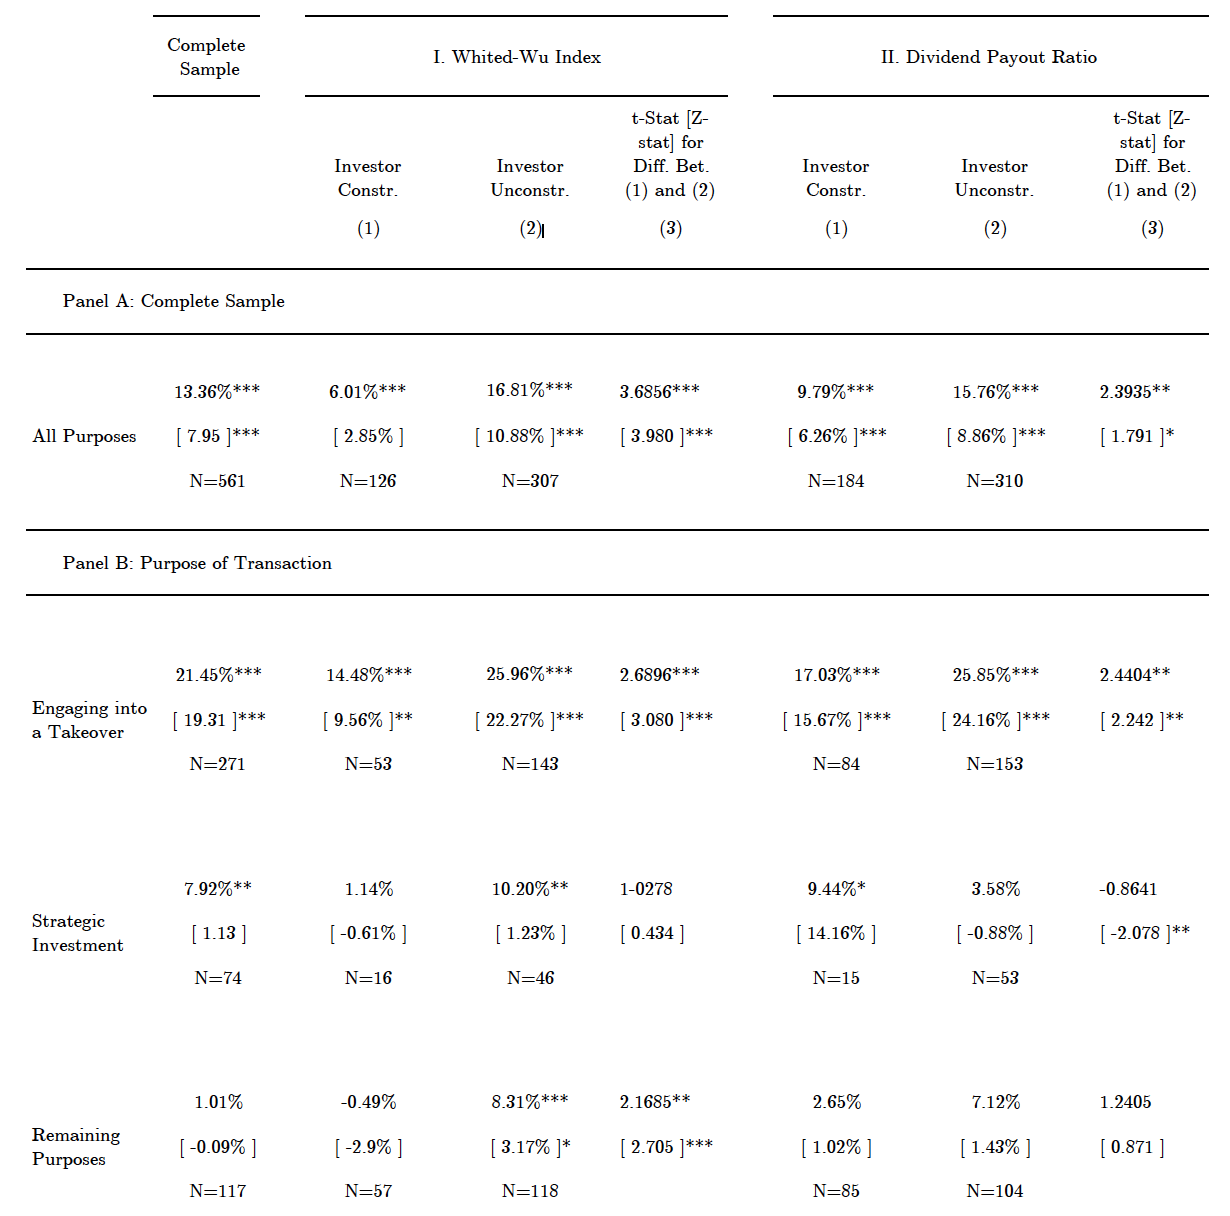
\includegraphics{Measures1}
	\end{adjustbox}\par\medskip
\end{table}

\pagebreak


\begin{table}[!htb]
	\centering
	\begin{adjustbox}{width=\textwidth}
		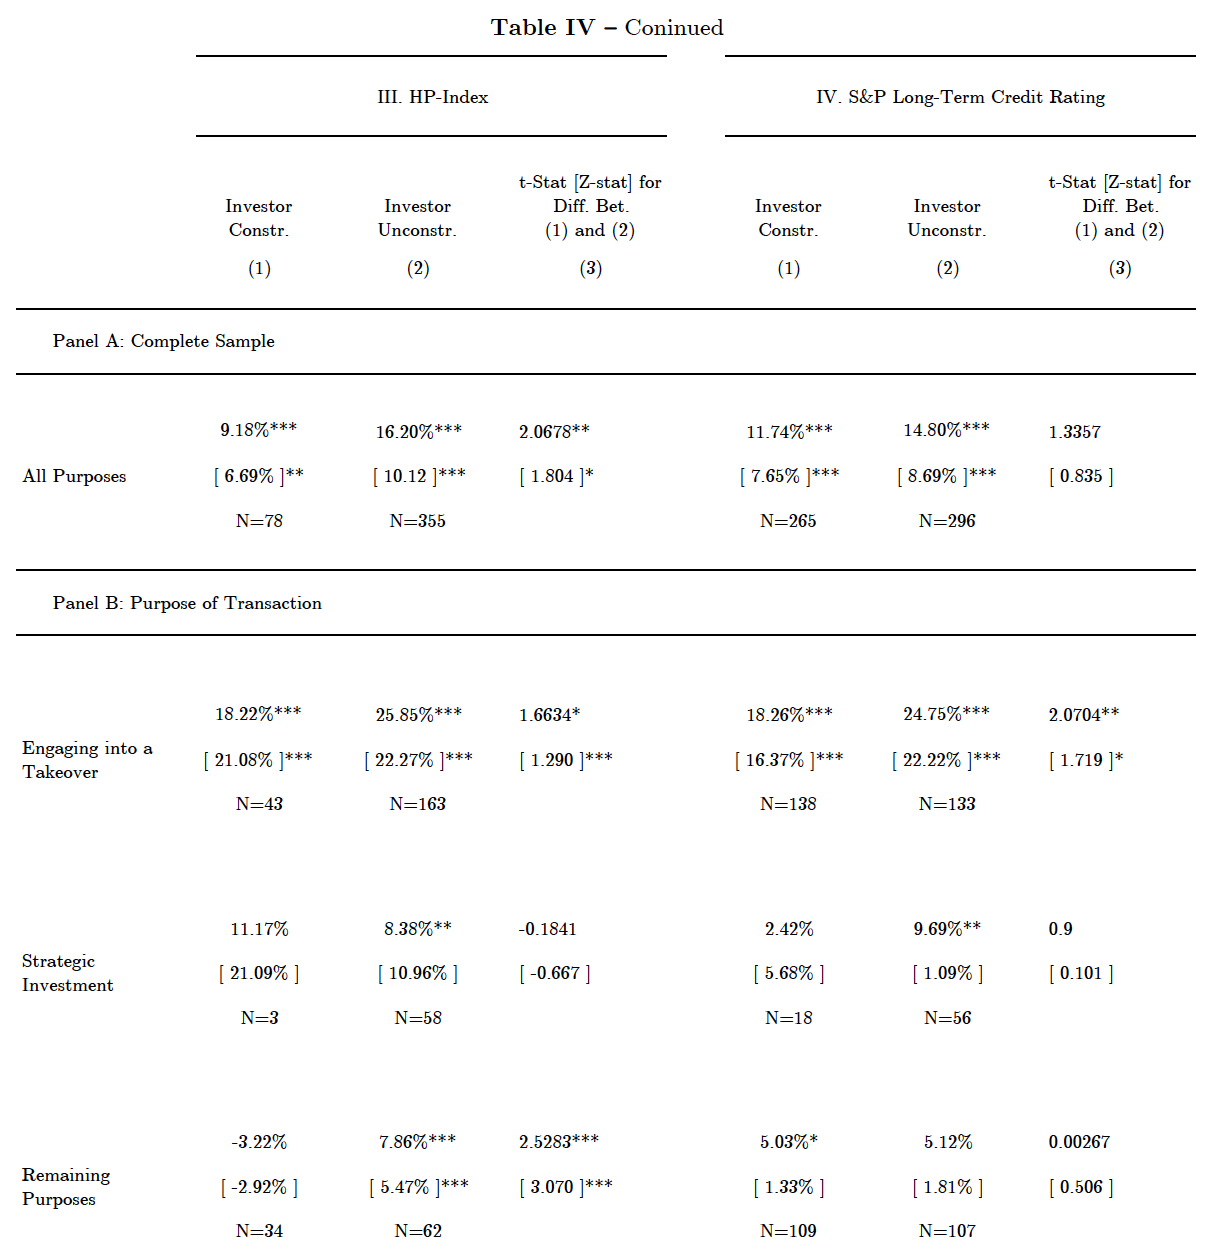
\includegraphics{Measures}
	\end{adjustbox}
\end{table}

\noindent Targets subject to filings with the purpose of strategic investments have a 7.92\% CAR, significant at the 5\% level which is a similar market reaction to the one observed by \citet[p.]{Allen2000} who finds abnormal returns of 6.9\% in response to strategic announcements. For the reason that the sample consists of only 74 filings having the purpose of a strategic investment, performing tests and deriving conclusions on the difference's economic and statistical significance is problematic. The issue becomes even more demanding when further splitting these filings into sub-samples for each measure, as they become smaller and tests loose their meaningfulness. Subsequently, there are only 16, 15 and 18 observations in the three samples of constrained investors from the WW-Index, dividend payout ratio and credit rating and just three for the HP-Index. Samples of the Whited-Wu index and the investor's credit rating present differences in mean CAR's matching with previous findings but when considering the sub-samples of the dividend payout ratio and the HP-Index, results differ. Although for these, targets of constrained investors now have higher abnormal returns, the difference is not significant. Hence the samples small scales do not allow valid inferences between returns for targets of financially constrained and unconstrained investors.
For the remaining purposes, the sample size is large enough to draw univariate conclusions. As the average cumulative abnormal return during the [-10,3] event window for all remaining purposes is only 1.01\%,  filings disclosed for strategic investments and takeovers lead to the strongest market reactions. When looking at the abnormal returns for sub-samples of the Whited-Wu index, targets of constrained investors earn -0.49\% and those of unconstrained investors 8.31\%. The average CAR for targets of unconstrained investors is significantly different from zero plus the difference in abnormal returns is significant at the 5\% level. Similar conclusions can be drawn for the sub-samples formed according to the HP-index for which targets of constrained investor experience negative abnormal returns of -3.22\% and those of unconstrained investor 7.86\%. The difference average cumulative abnormal returns accross the two groups is significant at the 1\% level. Those are the only two sub-samples in which negative returns occur which implies the market perceives these announcements as a decline in the target's value.
Concerning the dividend payout ratio, the difference in mean CAR's is visible but not significantly different from zero and for the finishing with the samples of the credit rating, the difference is non-existent. 

The univariate analysis shows that both, across measures and transaction purposes, the difference in abnormal returns for targets of constrained investors is generally present and significant. Hence Table III gives further evidence on whether financial constraints of corporate activists matter. Irregularities are only evident for filings with the purpose of a strategic investment, but here too does the Whited-Wu index show differences in abnormal returns. 
Table III also shows that abnormal returns are the highest for filings with the purpose of engaging into a takeover, followed by filings disclosed due to a strategic investment. Except for these filings, statistical tests on differences are valid and show that the average CAR significantly differs across groups. Concluding, measures for identifying financially constrained investors separate the sample in a meaningful way and have categorical power when analyzing the sample's cumulative abnormal returns. This in turn supports the hypothesis that financial constraints of corporate activist investors matter. 

% The difference is the greatest among targets of constrained and unconstrained investors and of those missing a credit rating and those having one. For both measure, the difference is statistically significant at the 1\% level. Strikingly, targets of investor identified to be in financial distress have a mean CAR of 25.65\%, 4\% higher when compared to undistressed firms. An explanation might be that the distressed companies equity claimants are up for a "gamble of ressurection" \citep[p.451]{Bhagat2005} in which they hope conditions may improve and the market interprets this behavior as promising for the target. For all measures, excluding the $Z$-score, is the difference in abnormal returns between the two sub-samples statistically significant at the 1\% level and targets of investor in the favorable state gain more

\section{Cross Sectional Variation of Abnormal Returns}

Equally important as the average abnormal return subject of analysis in the previous section is its cross-sectional variation because it reflects the heterogeneity in market perceptions regarding the expected value generated by activism. The advantage is that it allows to draw \emph{ceteris paribus} conclusions, which simple t-tests of means cannot do \citep[p.111]{Khatami2014}. Does the market's perceived value improvement for the target depend on the investor? What is the relationship between financially constrained investors and target's abnormal returns among the sample of Schedule 13(D) filings? Table V reports the results from regressions exploring the cross-sectional variation in market response to corporate investor activism. The regression is constructed as follows 

\begin{equation}
	AR_{i}=\beta_{0}+\beta_{1}FC_{i}+\sum_{k=1}^{n}\beta_{k}+X_{k,i}+\epsilon_{i}
\end{equation}
where the dependent variable $AR_{i}$ is the cumulative abnormal return in the [-10,3] and [-1,3] event window for target $i$. FC is a dummy variable equal to 1 if in filing $i$ the investor is classified as financially constrained and zero if otherwise and corresponds to each of the measures. For each classification -- Whited-Wu index, HP-Index dividend payout ratio and credit rating, the regression is performed separately. $X_{k,i}$ represents a vector of control variables of filing, investor and target characteristics, with \emph{takeover} and \emph{strategic} being equal to one if the transaction purpose was due to engaging into a takeover or strategic investment.  To minimize the risk of spurious inference, proxies for the business cycle \emph{recession}, and the investor's Tobin's Q are included. In addition, the regression controls for the \emph{ROA} and \emph{Cash flow from Operations to Assets} for both investor and target and the \emph{Relative Size}, defined as the natural logarithm of target total assets divided by bidder total assets. In a last step, all regressions control for the investor's industry, defined according to Fama \& French's 17 Industry classification code.\footnote{To prevent over-classification of the model, the 17 rather than the 48 industry classification is used.} 

\begin{table}
	\centering
	\captionsetup{textformat=empty,labelformat=blank}
	\caption{Relation between Abnormal Return and Financial Constraints}
	\begin{adjustbox}{max width=\textwidth}
		\begin{tabular}{lcccccccc}
			\multicolumn{9}{c}{Constraints} \\ \hline
			 & (1) & (2) & (3) & (4) & (5) & (6) & (7) & (8) \\
			VARIABLES &  \\ \hline
			 &  &  &  &  &  &  &  &  \\
			Whited-Wu Index & -0.1012*** &  &  &  & -0.0340** &  &  &  \\
			 & (-3.1909) &  &  &  & (-2.0327) &  &  &  \\
			hp\_indicator\_3 &  & -0.0264 &  &  &  & -0.0116 &  &  \\
			 &  & (-0.6352) &  &  &  & (-0.5479) &  &  \\
			Dividend Payout Ratio &  &  & -0.0447* &  &  &  & -0.0024 &  \\
			 &  &  & (-1.7344) &  &  &  & (-0.1882) &  \\
			rating\_indicator &  &  &  & -0.0037 &  &  &  & 0.0193* \\
			 &  &  &  & (-0.1425) &  &  &  & (1.6855) \\
			relsize & -0.2803*** & -0.2541*** & -0.2734*** & -0.3038*** & -0.0511 & -0.0138 & -0.0459 & -0.0624* \\
			 & (-4.3565) & (-3.9225) & (-4.6737) & (-5.2627) & (-1.4509) & (-0.3099) & (-1.3701) & (-1.8600) \\
			takeover & 0.1635*** & 0.1857*** & 0.1691*** & 0.1597*** & 0.0126 & 0.0137 & 0.0068 & 0.0043 \\
			 & (5.8778) & (6.5362) & (6.4145) & (6.6681) & (1.0206) & (0.9803) & (0.5273) & (0.3782) \\
			strategic & 0.0215 & 0.0440 & -0.0100 & 0.0272 & 0.0238 & 0.0289 & 0.0141 & 0.0278 \\
			 & (0.4372) & (0.9104) & (-0.2562) & (0.6328) & (0.7792) & (0.9230) & (0.5003) & (1.0699) \\
			recession & 0.0433 & 0.0216 & -0.0077 & 0.0009 & -0.0058 & -0.0040 & -0.0070 & -0.0152 \\
			 & (1.1501) & (0.5951) & (-0.2381) & (0.0297) & (-0.3986) & (-0.2692) & (-0.5429) & (-1.2534) \\
			CF from Operations / Assets & -0.0135 & 0.2189 & 0.1333 & 0.2431 & 0.2222** & 0.2282** & 0.2107*** & 0.2083*** \\
			 & (-0.0557) & (1.1638) & (0.8223) & (1.5693) & (2.1552) & (2.3739) & (2.6552) & (3.0030) \\
			CF from Operations / Assets (Target) & 0.1949** & 0.0522 & 0.0690 & -0.0825 & 0.0736** & 0.0742** & 0.0652** & 0.0289 \\
			 & (1.9948) & (0.5188) & (0.6959) & (-0.7601) & (2.0214) & (2.2200) & (2.0647) & (0.8392) \\
			Tobin's Q & -0.0038 & -0.0055 & -0.0086 & -0.0019 & -0.0064 & -0.0093 & -0.0106 & -0.0092 \\
			 & (-0.3218) & (-0.5291) & (-0.8022) & (-0.2082) & (-0.9221) & (-1.2768) & (-1.6349) & (-1.6448) \\
			Tobin's Q (Target) & -0.0232*** & -0.0279*** & -0.0243*** & -0.0261*** & -0.0047 & -0.0076 & -0.0083** & -0.0069* \\
			 & (-3.6815) & (-3.8742) & (-4.0870) & (-4.3028) & (-1.1280) & (-1.6418) & (-2.1867) & (-1.8040) \\
			ROA & -0.1419 & -0.2760 & -0.1537 & -0.2657* & -0.2249** & -0.2102** & -0.1828** & -0.1664** \\
			 & (-0.6171) & (-1.3470) & (-0.9216) & (-1.6641) & (-1.9719) & (-2.0753) & (-2.0664) & (-2.1507) \\
			ROA (Target) & -0.2451** & -0.0445 & -0.0741 & 0.0859 & -0.1047** & -0.1037** & -0.0866* & -0.0501 \\
			 & (-1.9925) & (-0.3643) & (-0.6216) & (0.7231) & (-2.0825) & (-2.2350) & (-1.9544) & (-1.1541) \\
			 \\
			 &  &  &  &  &  &  &  &  \\
			Constant & 0.2887*** & 0.2188*** & 0.2629*** & 0.2390*** & 0.0808* & 0.0550 & 0.0846** & 0.0759* \\
			 & (3.9297) & (2.9130) & (3.4050) & (3.2169) & (1.7462) & (1.1047) & (1.9890) & (1.9183) \\
			 &  &  &  &  &  &  &  &  \\
			Observations & 401 & 403 & 458 & 521 & 401 & 403 & 458 & 521 \\
			 R-squared & 0.2553 & 0.2482 & 0.2360 & 0.2170 & 0.1248 & 0.1108 & 0.1041 & 0.1012 \\ \hline
			\multicolumn{9}{c}{ Robust t-statistics in parentheses} \\
			\multicolumn{9}{c}{ *** p$<$0.01, ** p$<$0.05, * p$<$0.1} \\
			\end{tabular}			
	\end{adjustbox}
\end{table}
Turning first to column (1) and keeping everything else equal, corporate activism of Whited-Wu-financially constrained investors generates abnormal returns 10.12\% lower when compared to activism by unconstrained investors. The coefficient of the Whited-Wu dummy variable is significant at the 1\% level, implying that investor's financial constraints matter when the market reacts to Schedule 13(D)filings and there is cross-sectional dependency between abnormal returns and the investor's financial condition. Furthermore, the relative size seems to be an important determinant of the market reaction, meaning that if investor and target have the same size, abnormal returns are reduced by 28\%. With a significant intercept of 22.84\% at the 1\% level this implies negative returns of -5\%, other things being equal. Because the regression controls for the investor's size, the effect of the financial constraints variable is independent from the size effect. This means that the Whited-Wu index not just identifies small investors as financially constrained but de facto uses different criteria. Furthermore, the dummy variable takeover has a positive coefficient of 16.35 which is significant the 1\% level. When compared to the coefficient of the variable strategic which is only 2.15, the results of the regression are matching with the previous analysis, namely that targets subject to filings with the purpose of engaging into a takeover experience the largest abnormal returns. Moreover the coefficient on cash flow from operations to assets from the target shows that the more profitable the target is, the higher are the abnormal returns. Interesting is the fact that the target's investment opportunity has a negative influence on the market's evaluation of the target as target's with a higher Tobin's Q have abnormal returns 2.3\% lower, all other things being equal.

Heading to Column (5), in which the [-1,3] CAR is the dependent variable, similar effects are shown. Targets of financially constrained investors have abnormal returns 3.4\% lower, which is significant at the 1\% level. As the intercept predicts abnormal returns of 8\%, a decrease in abnormal returns of 3.4\% is a big difference.

Column (2) and (6) show regression results using the HP-index as measure of financial constraints. Across both event windows, the coefficient points in the right direction of decreasing abnormal returns for constrained investors but is not significant. This might be due to its high correlation with the control variable relative size and the small amount of only 78 financially constrained investors according to this measure. Nonetheless, relative size, takeover, the target's Tobin's Q and ROA have similar effects as in the previous regressions.

Column (5) and (6) show regression results using the investors dividend payout as a dummy for financially constrained and unconstrained investors. In column (5), the coefficient is significant at the 10\% level, meaning that other things being equal, targets of constrained investors have abnormal returns 4.37\% lower when compared to those of unconstrained investors. This is further evidence that financial constraints of the investors do matter as there exists a cross-sectional relationship. Although, the coefficient of the dividend payout ratio looses its significance in the shorter event window [-1,3], the sign of the coefficient points in the right direction. As the coefficient looses its significance, investor's cash flow from operations and return on assets, hence profitability, becomes an important. Other things equal, the higher the investor's profitability, the higher are the target's abnormal returns. While not providing evidence on financial constraints, it further shows that the investor's health and financial independence are determining factors. 
The last two regressions in column (4) and (8) include the investor's rating as a dummy for constrained and unconstrained investors. Similar to the HP-Indicator, the investor's credit rating has no cross-sectional significance in explaining the target's cumulative abnormal returns. Similarly, the correlation between the variable relative size and the dummy variable is strong as ratings and size of the investor proceed conjointly. Nonetheless, the exists no significant relation between the target's abnormal returns and the rating of the investor. Turning to column (8) the coefficient states that other things being equal, targets of investors missing a credit rating have abnormal returns 1.94\% higher, significant at the 10\% level. This is a contradiction to the previous results as it indicates that targets of financially constrained investors gain in the shorter window more, when compared to targets of unconstrained investors. - explanation - 

The multivariate analysis provides further evidence that financial constraints of investors could matter to the market when it evaluates the potential value increase for the target. The regressions show that other things being equal, target of financially constrained investors have abnormal returns significantly lower when compared to targets of unconstrained investors around the Schedule 13(D) filing date.  The meaningfulness of the cross-sectional analysis however is limited. Only two out of the four measures of financial constraints are significant and there exists variation among the two event windows. Nevertheless, the regressions provide further evidence and show that the financial constraints measures have explanatory power beyond the size-effect.


% \begin{table}[ht]
% 	\centering
% 	\caption{Constraint Measures}
% 	\begin{adjustbox}{max width=\textwidth}
% 		\begin{tabular}{lcccc}
% 			\multicolumn{5}{c}{Constraints} \\ \hline
% 			 & (1) & (2) & (3) & (4) \\
% 			VARIABLES \\ \hline
% 			 &  &  &  &  \\
% 			Whited-Wu Index & -0.0943*** &  &  &  \\
% 			 & (-2.9888) &  &  &  \\
% 			hp\_indicator\_2 &  & 0.0164 &  &  \\
% 			 &  & (0.3308) &  &  \\
% 			Dividend Payout Ratio &  &  & -0.0476* &  \\
% 			 &  &  & (-1.8782) &  \\
% 			rating\_indicator &  &  &  & -0.0010 \\
% 			 &  &  &  & (-0.0374) \\
% 			relsize & -0.2800*** & -0.2774*** & -0.2632*** & -0.2761*** \\
% 			 & (-4.2021) & (-4.3067) & (-4.5934) & (-4.5798) \\
% 			takeover & 0.1821*** & 0.1878*** & 0.2017*** & 0.1845*** \\
% 			 & (5.1027) & (5.3377) & (6.1235) & (6.2645) \\
% 			strategic & 0.0520 & 0.0549 & 0.0222 & 0.0436 \\
% 			 & (1.0199) & (1.0434) & (0.5148) & (0.9665) \\
% 			investment & 0.0523 & 0.0244 & 0.0757* & 0.0564 \\
% 			 & (1.1719) & (0.6240) & (1.9417) & (1.4550) \\
% 			recession & 0.0351 & 0.0027 & -0.0166 & -0.0008 \\
% 			 & (0.9178) & (0.0732) & (-0.5112) & (-0.0265) \\
% 			CF from Operations / Assets & -0.1676 & -0.0164 & -0.0163 & 0.0381 \\
% 			 & (-1.4711) & (-0.1684) & (-0.1572) & (0.3923) \\
% 			CF from Operations / Assets (Target) & 0.0106 & 0.0078 & 0.0121 & -0.0253 \\
% 			 & (0.1977) & (0.1543) & (0.2341) & (-0.4439) \\
% 			Tobin's Q & -0.0036 & -0.0106 & -0.0080 & -0.0043 \\
% 			 & (-0.3103) & (-0.9979) & (-0.7586) & (-0.4649) \\
% 			Tobin's Q (Target) & -0.0207*** & -0.0245*** & -0.0227*** & -0.0258*** \\
% 			 & (-3.3555) & (-3.6770) & (-3.8943) & (-4.2064) \\
% 			Fama-French industry code (17 industries) = 4, omitted & - & - & - & - \\
% 			 &  &  &  &  \\
% 			Constant & 0.2235*** & 0.2076** & 0.1993** & 0.1873** \\
% 			 & (2.6882) & (2.3870) & (2.4461) & (2.3371) \\
% 			 &  &  &  &  \\
% 			Observations & 401 & 398 & 458 & 521 \\
% 			 R-squared & 0.2509 & 0.2399 & 0.2404 & 0.2160 \\ \hline
% 			\multicolumn{5}{c}{ Robust t-statistics in parentheses} \\
% 			\multicolumn{5}{c}{ *** p$<$0.01, ** p$<$0.05, * p$<$0.1} \\
% 			\end{tabular}			
% 	\end{adjustbox}
% \end{table}

\section{Conclusion}

Schedule 13(D) filings enjoy wide spread attention, particularly when initiated by institutional investors. Recent literature has addressed their interests and motives, the value added and highlighted differences across investor types. Yet a detailed investigation of corporate activist investors has not been conducted. This thesis supports the evidence on why corporations would actively hold equity ownership, namely in the process of takeovers, strategic investments and issuer financing. Furthermore, targets of corporate activist investors experience significant gains around the filing date of a Schedule 13(D). In fact, the general sample experiences average abnormal returns of 13\%. This is in line with existing evidence that activism -- in any form -- is perceived as an actual value improvement for the target. 
Furthermore, using a sample of Schedule 13(D) filings disclosed by corporations from the period 1996-2016, the effect of investor's financial constraints on target's gains is analyzed. The thesis provides evidence that financial constraints of activist investors matter, as in the manifestation of significantly lower abnormal returns for targets of financially constrained investors. Across all purposes and independent of the financial constraints measure, these targets have much smaller abnormal returns. The evidence is further supported by the cross sectional analysis of stock returns, showing that the financial constraints of corporate activists matter. Other things equal, targets of constrained investors have abnormal returns 10\% lower when compared to those of unconstrained investors. Concluding, both univariate and multivariate analysis show, that financial constraints of corporate activist investors matter. 
% As this thesis seeks to explore the relation between the filing of a Schedule 13(D) and the investor's financial condition, the event window (-1,3) is used for all following analysis. This is done for two reasons. During the window [-10,3] the targets' abnormal returns experience two jumps, one at day minus 7 and the second at the filing day. This proves that the filing has an impact on the market and precisely this effect is subject of analysis. The second reason for choosing the event window (-1,3) is that regardless from Graph 1, the actual filing happens on day 0 and not on day -7 and therefore the abnormal returns close to day 0 should be importance. One disadvantage of this approach is, that leakage of information prior to the filing is left outside and aggregated returns have a downward bias.

\pagebreak

\begin{comment}
	
\section{Indentifying the Financial Condition of the Investor}
% Objective -- What is the financial condition? 
% Topics: Composition | Elements | Procedure
 

\subsection{Piotroskis F-Score -- A Measurement of Financial Strength}
%Objective -- How do we characterized strong firms? 
%Topics: Descrription | Why | Outlook 

In a study of 2010, \emph{BCG} noted many of that year's acquisitions would involve a financially strong acquirer. However, the attribute of being financially strong is not ambivalent. Piotroski's F-Score adresses this issue as it is a "... composite measure of firm strength" \citep[p. 496]{Fama2006}. It consists of nine binary signals which consider in what directions the fundamentals of a company are trending and whether general health conditions are met \citep{Mohr2012}. \citet{Piotroski2000} established it to seperate strong from weak value firms
	\footnote{In order to legitimize the explanatory power of the F-score in separating strong from weak firms Piotroski formed portfolios consisting of value firms. In doing so, he showed that an investment strategy of shorting expected losers (weak firms) and buying expected winners (strong firms) would "generate a 23\% average annual return" \citep[p. 4]{Piotroski2000}. This is matching with \citet{Hyde2014} results, who observe significant return premiums for stocks with a high F-score over stocks with a low F-score.}
. 
Although the F-score was established to distinguish among value firms, \citet{Mohr2012} shows that its application on growth stocks yields similar results.
	\footnote{This is in line with \citet{Piotroski2000} and confirms earlier research conducted by him.}. 
With regards to the above, the F-Score is used to divide the complete sample of investors into strong and weak ones.

\subsection{The Whited-Wu Index -- A Measurement of Financial Constraints}
A firm is financially constrained if it faces an inelastic supply of external capital \citep{Farre-mensa2013} and those who are able to raise substential amounts of external capital without much of an increase in the cost of capital are unconstrained. Although \citet{Khatami2014} notes that more recent literature has questioned the reliability of constraint measures, the Whited-Wu Index as in \citet{Liao2010} is used as an indicator. 


\subsection{Altman's Z-Score -- A Measurement of Financial Distress}
Financial distress describes a state in which a company cannot meet or has difficulty paying off, its financial obligatiosn to its creditors. In this sense, HNA Group could be in a state of financial distress as they have problems refinancing the debt burden, and recently planned to sell their stake in Hilton Worldwide Holdings Inc. to pay down a large pile of debt. Altman's Z-score is a widely accepted measure of financial distress. The fundamental indicator shows statistically significant results in predicting the bankruptcy of a company \citep{Campbell2008} and is still applied as a general practical tool for assessing the financial well-being of firms \citep{Kleinert2014}. 
	\footnote{The model consists of five financial ratios that are coefficients by discriminate analysis method where the financial ratios are independent variables of it. The five financial ratios of the Z-score are (1) working capital to total assets, (2) retained earning to total assets, (3) earnings before interest and taxes to total assets, (4) market value of equity to book value total debt and (5) sales to total assets. This yields
		\begin{equation}
			Z=1.2(X_{1})+1.4(X_{2})+3.3(X_{3})+0.6(X_{4})+0.999(X_{5})
		\end{equation}
	The cut-off point is at Z=2.675 where a lower score implies bankruptcy of a firm and a higher score non-bankruptcy.}
.

\subsection{Other Measurements}

\subsection{Tobin's Q}
Tobin's Q is included because it proxies for a firm's investment opportunity which assesses the 
\footnote{In accordance with \citet{Brigida2012}, Tobin's Q is defined as 
\begin{equation}
	Tobin's Q= \frac{MVE + PSE + Debt}{AT}
\end{equation}, where $MVE$ is the market capitalization, $PSE$ is the lquidating value of preferred stock, $Debt$.. } 
\citep{DUCHIN2010}. According to \citet{Khatami2014} constrained firms have higher tobin's Q compared to unconstrained firms, which may be due to their unexploted investment opportunities \citep{Khatami2014}.

\subsection{Company Size}
Company size 



\pagebreak

It was established by Altman in his 1968 paper 


In conducting the analysis, the F-score will be used to separate  the sample of 13D filings among strong and weak corporate investors. Since is is able to separate firms in portfolios into strong and weak performing ones, an application to this analysis seems reasonable. 
%insert negative aspects here - accruals 
However, components of the f-score include changes in leverage and The score itself can be divided into the three dimensions profitability, balance sheet health and operating efficiency. 
In the context of this analysis As \citet{Mohr2012} states: the f-score considers in what direction the fundamentals of a company are trending and whether financial health conditions are met.  Because high F-scores imply higher returns hence stronger firms should have higher returns, investors must see a high F-score as a representation of financial strength. In the context of this paper those practices would have only been applied to the target and not the investor. An application of the F-score on the investor with the aim of distinguishing between strong and weak firms 


\citet{Choi2012} formulate it from a target perspective - "does financial strength predict subsequent institutional demand"? 

%In general, analyzed characteristics across the sample of filings but not the characteristics of the parties in general.

On the other hand, \citet{Akhigbe2007} examine the characteristics of final acquisitions following partial bids. They find that involvements by corporate bidders are more likely to result in a full acquisition. 

% previous studies have examined the content of the filings and therefre indirectly involved the investor in their analysis and when actively invo lving a party only analysed the target (s. above paragraph).
% difference of the paper 
\end{comment}
\pagenumbering{roman}
\begin{appendices}
	\renewcommand{\appendixname}{Appendix}

	\section{Financial Constraints Measures \& Variables}

	\subsection*{Whited--Wu Index}
	\noindent Used from \citet[p.543]{Whited2006} and following \citet[p.38]{Farre-mensa2013} the Whited-Wu index is calculated as:
		\begin{equation*}
		WW=-0.091X_{1}-0.062X_{2}+0.021X_{3}-0.044X_{4}+0.102X_{5}-0.035X_{6}
		\end{equation*}
	where
	\begin{itemize}
	\renewcommand\labelitemi{}
		\item $X_{1}$ is the ratio of cash flow to assets defined as the sum of income before extraordinary items and depreciation and amortization divided by total assets $\frac{ib+dp}{at}$
		\item $X_{2}$ is an indicator set to one if the firm pays a dividend, likewise if the sum of common and preferred dividends paid is positive, zero otherwise $dvp+dvc>0$
		\item $X_{3}$ is the ratio of long-term debt to total assets $\frac{dltt}{at}$
		\item $X_{4}$ is the size of the investor defined as the natural logarithm of total assets $log(at)$
		\item $X_{5}$ is the average industry sales growth, estimated for each three digit SIC industry and each year separately $\frac{SALE_{t}}{SALE_{t-1}}$
		\item $X_{6}$ is the investor's sales growth $\frac{SALE}{SALE_{t-1}}$
	\end{itemize}

	\noindent Following convention, the index is calculated for all firms on Compustat and firms are then sorted into terciles based on their index value. Firms in the top tercile are coded as constrained and those in the bottom tercile are coded as unconstrained \citep[p.38]{Farre-mensa2013}. 

	\subsection*{Dividend Payout Ratio}
	\noindent Following \citet[p.119]{Khatami2014} and \citet[p.1789]{Almeida2004}, the investor's dividend payout ratio is defined as the two-year average of the dividend payout ratio from the two preceeding annual reports at each point in time.\\
	The yearly dividend payout ratio is defined as the sum of dividends ($dvp+dvc$) plus stock repurchases (total expenditure on the purchase of common and preferred stocks $prstkc$) minus any reduction in the value of net number of preferred stocks outstanding (redemption value $pstkrv$) divided by operating income ($\frac{ib}{at}$) as in \citet[p.369]{Jagannathan2000}. Further, following \citet[p.119]{Khatami2014} and \citet[p.1923]{hadlock2010} dividend payout ratios are set equal to 1 if they are above 1 and if a firm has negative operating income and positive dividends. After computing the two-year average payout ratio for all firms on Compustat, firms are sorted into terciles based on their annual payout distribution. Firms in the bottom (top) tercile are coded constrained (unconstrained). 

	\subsection*{HP / SA -- Index}
	\noindent Following \citet[p.1929]{hadlock2010} and \citet[p.119]{Khatami2014} the index is calculated as: $HP=-0.737*Size+0.043*Size^{2}-0.040*Age$ where size is the log of inflation adjusted (to 2004) book assets and age is the number of years the firm has been on Compustat with a non-missing stock price. In calculating the index, size is replaced with log(\$4.5 billion) and age with 37 years if the actual values exceed these thresholds \citep[p.1929]{hadlock2010}. After computing the HP index for all companies on Compustat, the firms are sorted into terciles based on their annual index values. Firms in the top tercile are coded as constrained and those in the bottom tercile are conded as unconstrained \citep[p.38]{Farre-mensa2013}.
	\pagebreak

	\subsection*{Other Variables}

	\begin{itemize}
	\renewcommand\labelitemi{--}
		\item Return on assets $\frac{ebitda}{at}$
		\item Cash flow from operations to total assets $\frac{oancf}{at}$
		\item Cash and short-term investments to total assets $\frac{che}{at}$
		\item Cash to total assets $\frac{ch}{at}$
		\item Book Leverage \citep[p.1440]{MacKay2005} $\frac{dltt+dlc}{at}$
		\item Short-term debt to total assets $\frac{dlc}{at}$ 
		\item Long-term debt to total assets $\frac{dltt}{at}$
		\item Market value of equity $prcc_f*csho$
		\item Size of the firm $log(at)$
		\item Tobin's Q \citep[p.120]{Khatami2014} $\frac{at-ceq-txdb+csho*prcc_c}{at}$
	\end{itemize}

\section{Categorization of Purpose of Transaction}

\noindent The following definitions are explanatory excerpts of Schedule 13(D) filings from the sample. Based on these descriptions the filing's transaction purpose was identified. Following, the Reporting Person is the investor disclosing the Schedule 13(D) wheras the Issuer is the company subject to the filing. 
\begin{enumerate}
	

\item Merger: "the Company entered into the Merger Agreement with the Reporting Person and Merger Sub, pursuant to which the Reporting Person will acquire all of the outstanding equity interests of the Company."

\item Tender Offer: "The Reporting Person announced its intention to commence a partial cash tender offer for up to \emph{number of} shares of Common Stock at a price of \emph{\$ price} net per share"

\item Hostile Takeover: "The Shares have been acquired by the Reporting Persons with a view to ultimately acquiring  control of the Issuer  pursuant to a merger with, or  acquisition of additional  stock  by,  the Reporting Person  or one of its  subsidiaries. [...]
% Such  merger  or acquisition would likely result in changes to the present Board of Directors and management  of the  Company,  and  might  result  in  changes  in the  Company's capitalization and dividend policy, business, corporate structure and governing documents. 
The Reporting Person has contacted the Chairman of the Board of the Issuer and expressed an interest in acquiring the Company and expects to have further discussions  with management of the Issuer."

\item Investment Opportunity while Actively Monitoring the Target: "The primary purpose of the Reporting Person's acquisition of the Common Stock is for investment. The Reporting Person believes that at this time, the Common Stock represents an attractive investment opportunity. Although it has no current intention to do so, at some time in the future the Reporting Person may decide that it is desirable to seek to acquire the Issuer or seek to control or otherwise influence the management and policies of the Issuer."

\item Alliance Agreement: "The purpose of the transaction is for investment and to establish a long term distribution alliance between the Reporting Person and the Issuer."

\item License Agreement: "As set forth, the Shares were purchased on  in connection with the Development and License Agreement between the Issuer and the Reporting Person."

\item Joint Venture: "The Reporting Person acquired shared voting and investment power over the Contributed Shares in connection with the formation of the joint venture with the Issuer."

\item Engaging into a Proxy Fight: [...] nominating \emph{Person} and \emph{Person} to be elected by holders of the Shares to the Board of Directors of the Issuer (the “Board”) at the annual meeting of stockholders of the Issuer, or any other meeting of stockholders held in lieu thereof, and any adjournments, postponements, reschedulings or continuations thereof (the “Annual Meeting”). The Reporting Persons reserve the right to take all action they deem appropriate to obtain Board representation. 

\item Investor is Subject to Merger: "At the effective time of the Merger (the “Effective Time”), the separate existence of Merger Sub will cease and the Reporting Person will continue as the Surviving corporation and as a wholly owned subsidiary of the Issuer. Each holder of outstanding common stock of the Reporting Person, par value \emph{\$ per share} will receive, in exchange for each share of the Reporting Person's Common Stock held by such holder, \emph{amount} of a share of the Issuer Common Stock (the “Exchange Ratio”).

\item Issuer Financing: "The purpose of the purchase of the Stock was to provide the Issuer with immediately available funds to address its urgent liquidity needs in exchange for an equity interest in the Issuer."
\end{enumerate}

\section{Event Study}

\noindent In order to compute the abnormal returns $AR_{i,t}$ for security $i$ at time $t$ in \eqref{eq:1} the market model is used. For the expected return it assumes a constant and linear relation between the observed returns $R_{i\tau}$ and the return of a market index $R_{m\tau}$. The parameters are estimated by ordinary least squares regressions based on estimation-window observations \citep[p.210]{Corrado2011}. The value-weighted NYSE/Amex/Nasdaq index from CRSP is used as the market return $R_{M\tau}$.

			\begin{equation*}
				R_{i,\tau}=\alpha_{i}+\beta_{i}R_{M,\tau}+\epsilon_{i,\tau}
			\end{equation*}
			with 
			\begin{equation*}
				E[\epsilon_{i,\tau}]=0
			\end{equation*}
			and 
			\begin{equation*}
				Var[\epsilon_{i,\tau}]=\sigma^2_{i,\tau}
			\end{equation*}
			This yields the abnormal return $AR_{i,\tau}$
			\begin{equation}
				AR_{i,\tau}=R_{i,\tau}-(\hat{\alpha_{i}}+\hat{\beta_{i}}R_{M,\tau})
			\end{equation}

\section{Hypotheses}

\begin{itemize}
\renewcommand\labelitemi{}
	\item \nth{1} Hypothesis: Financial constraints of corporate activist investors should matter to the market's perception of the actual value improvement for the target.
	\item \nth{2} Hypothesis: Schedule 13(D) filings disclosed by corporate activist investors are characterized by abnormal share price reactions for the target
	\item \nth{3}
\end{itemize}

\section{Stata Do-Files}
\end{appendices}
\printbibliography
 
\end{document}

\subsection{Appendix B -- Financial Condition Measures}

\subsubsection{F-Score}
Used from \citet{Piotroski2000} and calculated according to \citet{Fama2006} and \citet{Choi2012}. Each component contributes one point if the condition holds, zero otherwise. 

	\begin{enumerate}
		\item Positive net income before extraordinary $IB$ $$IB>0$$
		\item Positive cash flow from operations  $OANCF$-- all investors had a reported cash flow format of 7. Therefore $$OANCF>0$$
		\item Cash flow from operations is greater than net income $$OANCF>IB$$
		\item Growth in net income $IB$ scaled by total assets $AT$ from prior fiscal year end $$\frac{IB}{AT}$$
		\item Decrease in leverage from prior fiscal year end with leverage defined as the sum of long-term debt $DLTT$ and long-term debt due in one year $DD1$ $$\frac{DLTT+DD1}{AT}$$
		\item Increase in liquidity from prior fiscal year end with liquidity defined as the ratio of current assets $ACT$ to total liabilities $LCT$ $$\frac{ACT}{LCT}$$
		\item No new common or preferred stock issued $SSTk$ over the previous year $$SSTK=0$$
		\item Increase in gross margin from piror fiscal year end with gross margin defined as one minus the ratio of costs of goods sold $COGS$ to sales $SALE$ $$1-\frac{COGS}{SALE}$$
		\item Increase in asset turnover from prior fiscal year end with asset asset turnover defined as the ratio of sales $SALE$ to total assets at the beginning of the year $AT_{t-1}$ $$\frac{SALES}{AT_{t-1}}$$
	\end{enumerate}


\subsubsection{Z-Score}
The Z-score is computed according to \citet[p.549]{Altman1968} and \citet[p.14]{Altman2002}. For firms in manufacutring industries (SIC industries 2000-3999) the Z-score is $$Z=1.2X_{1}+1.4X_{2}+3.3X_{3}+0.6X_{4}+1.0X_{5}$$ where firms with a score below the threshold of 1.81 are considered as distressed and those above 2.99 as not distressed \citep[p.14]{Altman2002}.\\
For all remaining industries the Z-Score is $$Z=6.56X_{1}+3.26X_{2}+6.72X_{3}+1.05X_{4}$$	
where firms with a score smaller than 1.1 are considered as distressed \citep[p.18]{Altman2002} and firms with a score higher than 2.6 as not distressed \citep[p.175]{Sulub2014}.\\
With $X_{1}- X_{5}$ being \\
$X_{1}$ = Working capital to total assets $\frac{WCAP}{AT}$\\
$X_{2}$ = Retained earnings to total assets $\frac{RE}{AT}$\\
$X_{3}$ = Earnings before interest and taxes to total assets $\frac{EBIT}{AT}$\\
$X_{4}$ = Market value of equity to book value of total liabilities $\frac{PRCC_F*CSHO}{LT}$\\
$X_{5}$ = Sales to total assets $\frac{SALES}{AT}$




\subsection{Appendix C}


			
		\item Market Return Model -- The model is classified as the restricted market model with $\alpha_{i}=0$ and $\beta_{i}=1$. This means that there is no estimation window required and the abnormal return $AR_{i,\tau}$ is  simply the difference between the observed return $R_{i,\tau}$ and the value-weighted NYSE/Amex/Nasdaq   index return $R_{M\tau}$.

			\begin{equation}\label{eq:6}
				AR_{i,\tau}=R_{i,\tau}-R_{M,\tau}
			\end{equation}	
	\end{enumerate}
\pagebreak


